\documentclass{article}
\usepackage{graphicx}
\usepackage{float}
\usepackage{enumitem}
\usepackage{titlesec}
\usepackage{paralist}


\title{
    \begin{figure}[ht]
        \begin{center}
        
\includegraphics[width=0.6\columnwidth]{logo.png}
        \end{center}
    \end{figure}
    \textbf{The Hive Security Tool: A Scalable and Collaborative Platform for Security Incident Response} \\ % Title of the assignment
}

\author{
  \begin{tabular}{c}
    Sanju Basak (1805064) \\
    Md. Sayeed Hasan Ovi (1805065)\\
    Bangladesh University of Engineering and Technology
  \end{tabular}
}
\date{September 14, 2023}

\begin{document}
\maketitle

\section*{Introduction}
TheHive is a scalable Security Incident Response Platform, designed to make life easier for SOCs, CSIRTs, CERTs and any information security practitioner dealing with security incidents that need to be investigated and acted upon swiftly. It is an open source tool that is free to use, modify and share. It is written in Java and AngularJS and uses Elasticsearch to index and store data.

\section*{History}
TheHive was initially developed by Thomas Franco, a security analyst at CERT-EU. It was later released as an open source project in 2014. TheHive is now maintained by TheHive Project, a non-profit organization based in France.
It is currently used by many organizations around the world, including the NATO Computer Incident Response Capability (NCIRC) and the Computer Emergency Response Team of the European Union Institutions (CERT-EU)



\section*{Workflow of TheHive}
\begin{figure}[ht]
    \centering
    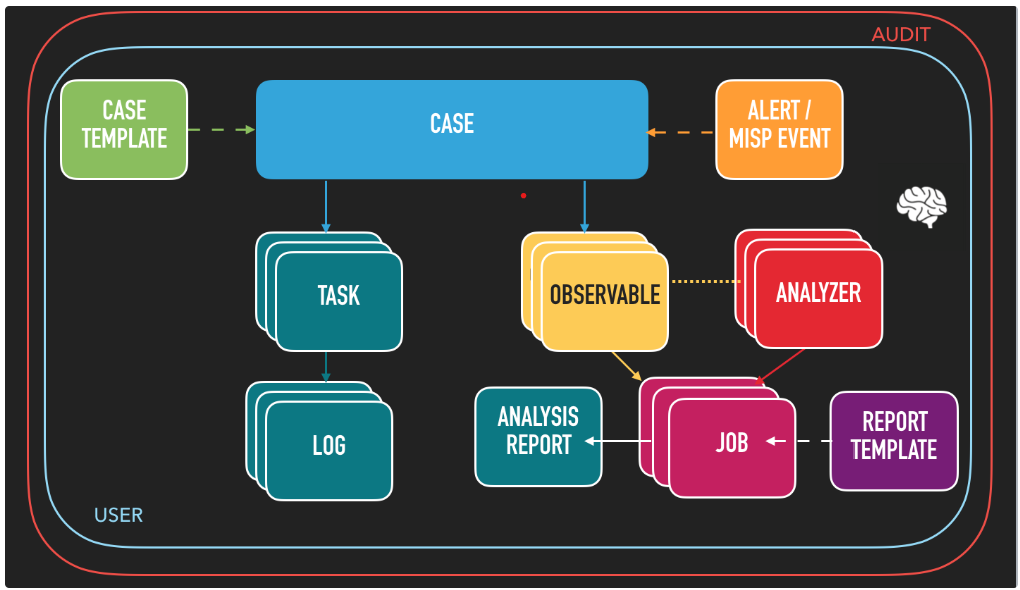
\includegraphics[width=0.8\textwidth]{workflow.png}
    \caption{Workflow of TheHive}
    \label{fig:workflow}
\end{figure}

TheHive workflow involves the following key steps:

\begin{itemize}
    \item \textbf{Create Case Template}: Create a case template to define the structure of incident cases. This includes the fields and attributes that will be used to document and manage incidents.

    \item \textbf{Create Case}: Document and manage incidents by creating cases. Assign cases to analysts or teams for resolution.

    \item \textbf{Create Tasks}: Assign tasks and responsibilities within cases to ensure organized incident response.

    \item \textbf{Create Alerts}: Create alerts to notify analysts of potential security incidents.

    \item \textbf{Create Observables}: Create observables to document and analyze potential threats associated with incidents.

    \item \textbf{Run Analyzers}: Use various analyzers to gather additional information and context about incidents and associated observables.

    \item \textbf{Create Logs}: Create logs to document actions taken by analysts during incident response.

    \item \textbf{Create Analysis Reports}: Use analysis reports to document findings and conclusions about incidents and observables.

    \item \textbf{Create Jobs}: Create jobs to automate incident response tasks.

    \item \textbf{Create Report Templates}: Create report templates to document incident response activities and outcomes.
\end{itemize}




\section*{Features}
TheHive has many features that make it a powerful tool for security incident response. Here we will discuss some of the most important ones.


\section{Admin side}
TheHive is a web application that can be installed on a server and accessed from a web browser. It has a web-based administration interface that allows administrators to configure the tool according to their needs. Administrators can create users, assign roles to them, and manage their permissions. They can also configure the tool to send notifications via email or SMS when certain events occur, such as new incidents being created or updated, or when certain actions are performed by users, such as adding comments or attachments to incidents.
list of features:
\begin{itemize}
\item Organization management
\item Link organizations
\item Account management
\item Entities 
\item Permission management
\item Observables types
\item Case Status
\item Alert Status
\end{itemize}

\subsubsection*{Organization management}
\subsection{Create an Organization}
TheHive allows administrators to create multiple organizations within the tool. Each organization can have its own set of users, roles, permissions, and notifications. This allows for better separation of duties and responsibilities between different teams within an organization, such as a SOC team and a CSIRT team.\\
To create a new organization, follow these steps: \\
\begin{enumerate}
    
\item Click on the \textbf{Add an Organization} button.
\item  Edit the required fields in the drawer:
    \begin{itemize}
        \item A placeholder exists and a logo of the Organisation can be added.
        \item Name: Name of the new Organization.
        \item Description: Description for the new Organization.
        \item Task sharing rule: default sharing rule for Tasks that will be applied when a Case will be shared with another Organization.
        \item Observables sharing rule: default sharing rule for Observables that will be applied when a Case will be shared with another Organization.
    \end{itemize}
\item  Click \textbf{Confirm} to create the organization.

\end{enumerate}

We can see this in Figure \ref{fig:org}.
\begin{figure}[ht]
    \centering
    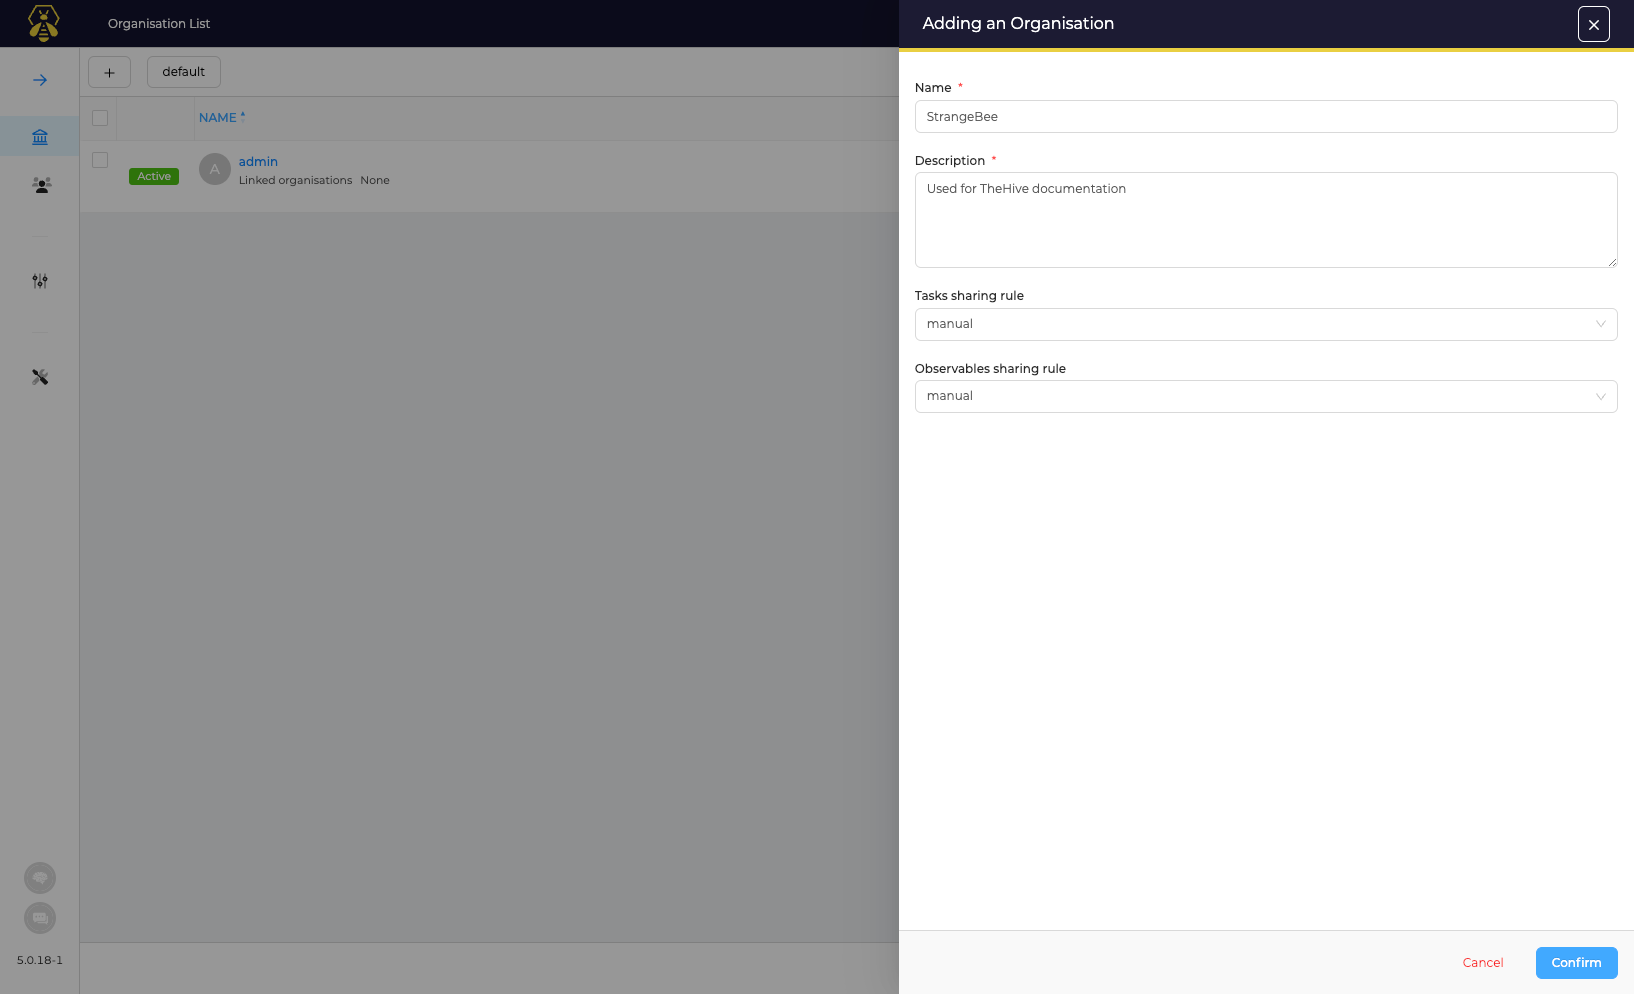
\includegraphics[width=0.8\textwidth]{organisations.png}
    \caption{Organization Management}
    \label{fig:org}
\end{figure}

\subsection{Link Organization}

TheHive allows administrators to link multiple organizations together. This allows for better collaboration between different teams within an organization, such as a SOC team and a CSIRT team.\\
To link an organization, follow these steps: \\

Here are the steps to manage links in TheHive:
\begin{enumerate}
    \item Open the detailed view of an Organization.
    \item Open the Linked Organization tab.



We can see this in Figure \ref{fig:link}.

\begin{figure}[H]
    \centering
    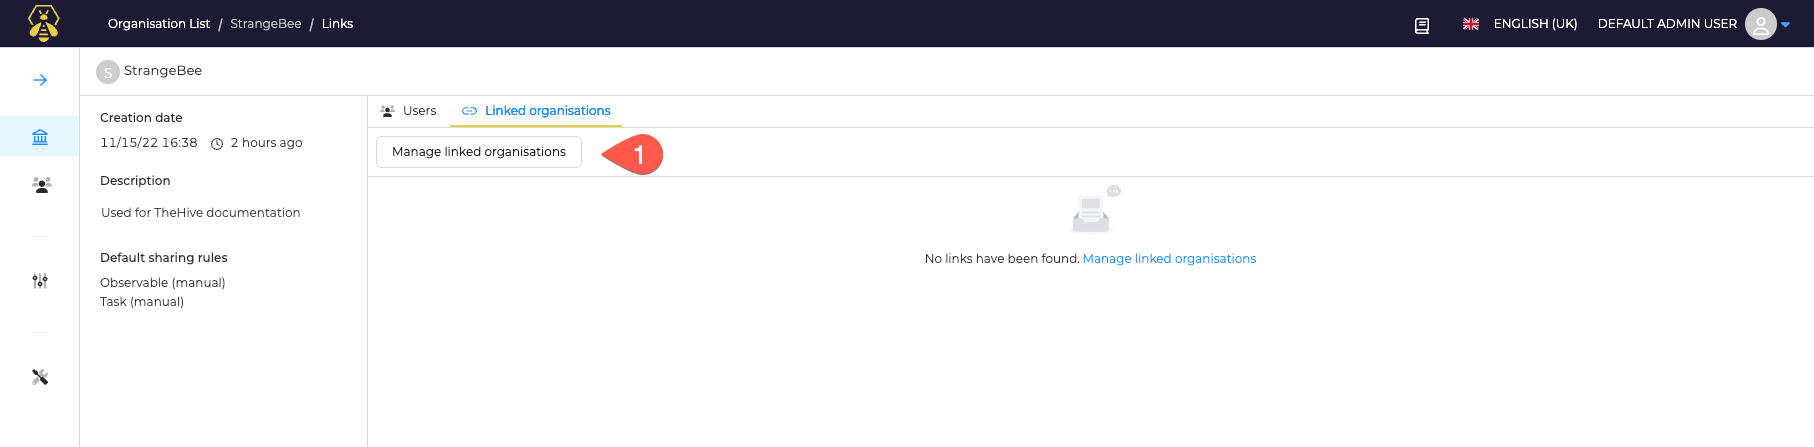
\includegraphics[width=0.8\textwidth]{organisation-links1.png}
    \caption{Link Organization}
    \label{fig:link}
\end{figure}
    \item  Click on the button named \textbf{Manage linked Organizations}.


We can see this in Figure \ref{fig:manage}.
\begin{figure}[H]
    \centering
    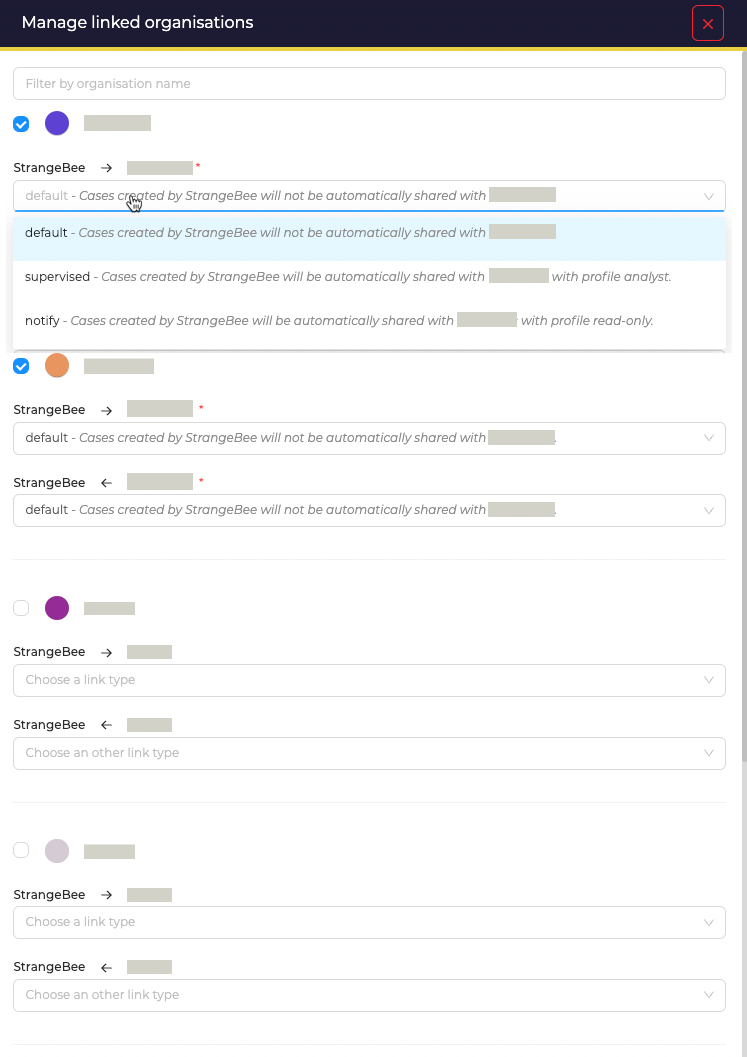
\includegraphics[width=0.8\textwidth]{organisation-links2.png}
    \caption{Manage Link Organization}
    \label{fig:manage}
\end{figure}

    \item For each other organization, select:
    \begin{itemize}
        \item If you want the current Organization to be linked with it.
        \item The types of link that should be created.
    \end{itemize}
\end{enumerate}

3 types of links are available:

\begin{itemize}
    \item default: Cases created by the current Organisation will not be shared with the other one.
    \item supervised: Cases created by the current Organisation will be automatically shared with the other one, with the profile Analyst.
    \item notify: Cases created by the current Organisation will be automatically shared with the other one, with the profile Read-only.
\end{itemize}

\subsection{Account Management}
TheHive allows administrators to create multiple user accounts within the tool. Each user account can have its own set of roles and permissions. This allows for better separation of duties and responsibilities between different users within an organization, such as a SOC team and a CSIRT team.\\
Accounts can be created or edited from several places in TheHive:

\begin{enumerate}
  \item As Administrator, in the Users view
  \item As Administrator in the detailed page of an Organisation
  \item As Org-admin, in the Organisation configuration page
  \item As Administrator of the platform, open the Users page.
\end{enumerate}

As Administrator of the platform, open the Users page. \\
We can see this in Figure \ref{fig:users}.
\begin{figure}[h!]
    \centering
    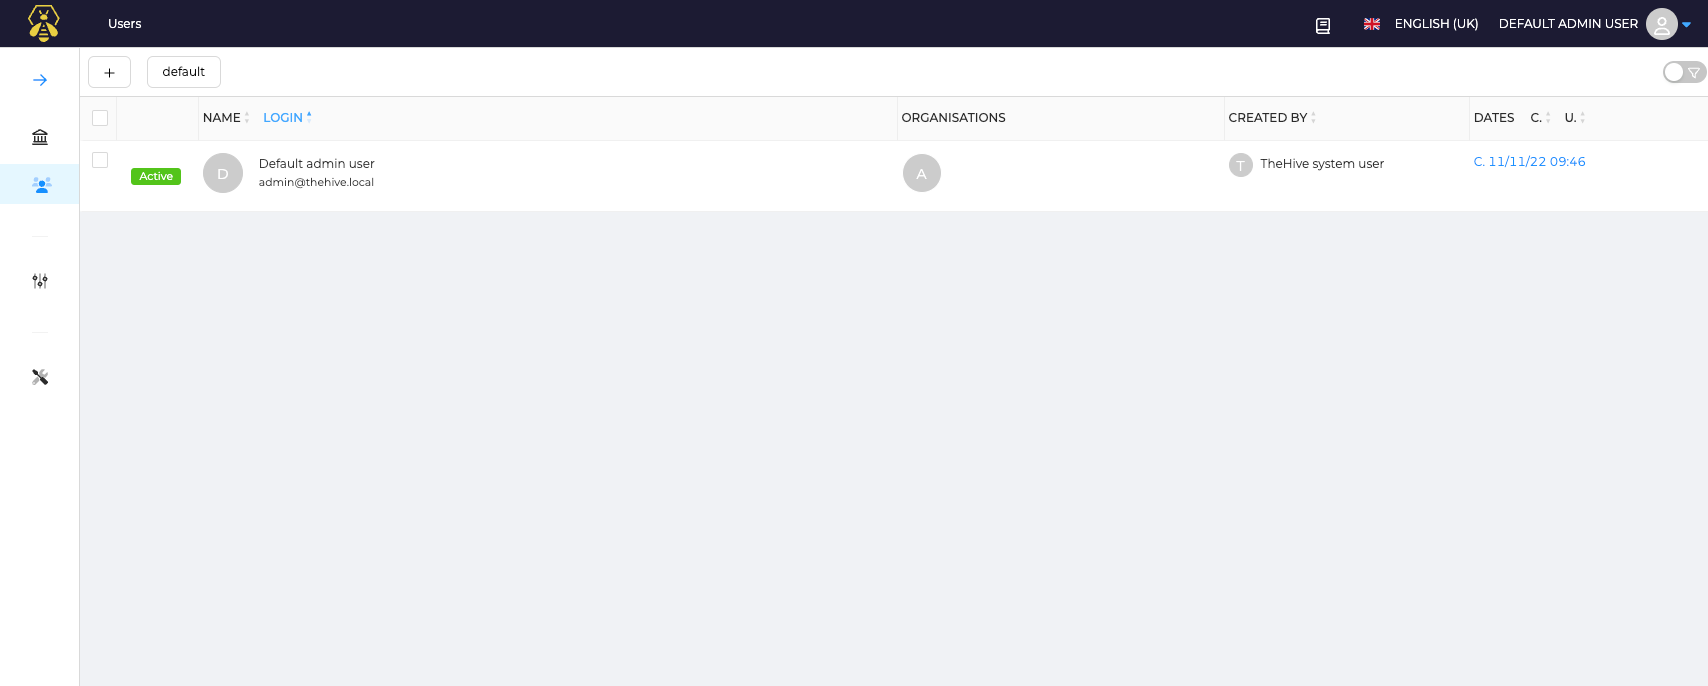
\includegraphics[width=0.8\textwidth]{accounts1.png}
    \caption{Users}
    \label{fig:users}
\end{figure}

Starting with TheHive 5.0, two types of accounts exist in the application:

\begin{enumerate}
  \item Normal accounts: These are used for standard users, such as analysts. These accounts can be used to open a session on the web UI, utilize all available authentication methods, and API keys if enabled.
  
  \item Service accounts: These are recommended for use by accounts in charge of automation within the application, such as those used to create Alerts. Service accounts can only be used to authenticate the application through the API, using an API key.
\end{enumerate}

Click on the \textbf{Add a User} button. \\
To create an account:

\begin{enumerate}
  \item Choose the type of account, either Normal or Service.
  \item Fill in the login name (formatted as an email address).
  \item Specify a name for the account.
  \item Select the organizations and associated profiles for this account.
  \item Click on "Set as default" to define the default organization for the account.
  \item Finally, click "Confirm."
\end{enumerate}

We can see this in Figure \ref{fig:add}.
\begin{figure}[h!]
    \centering
    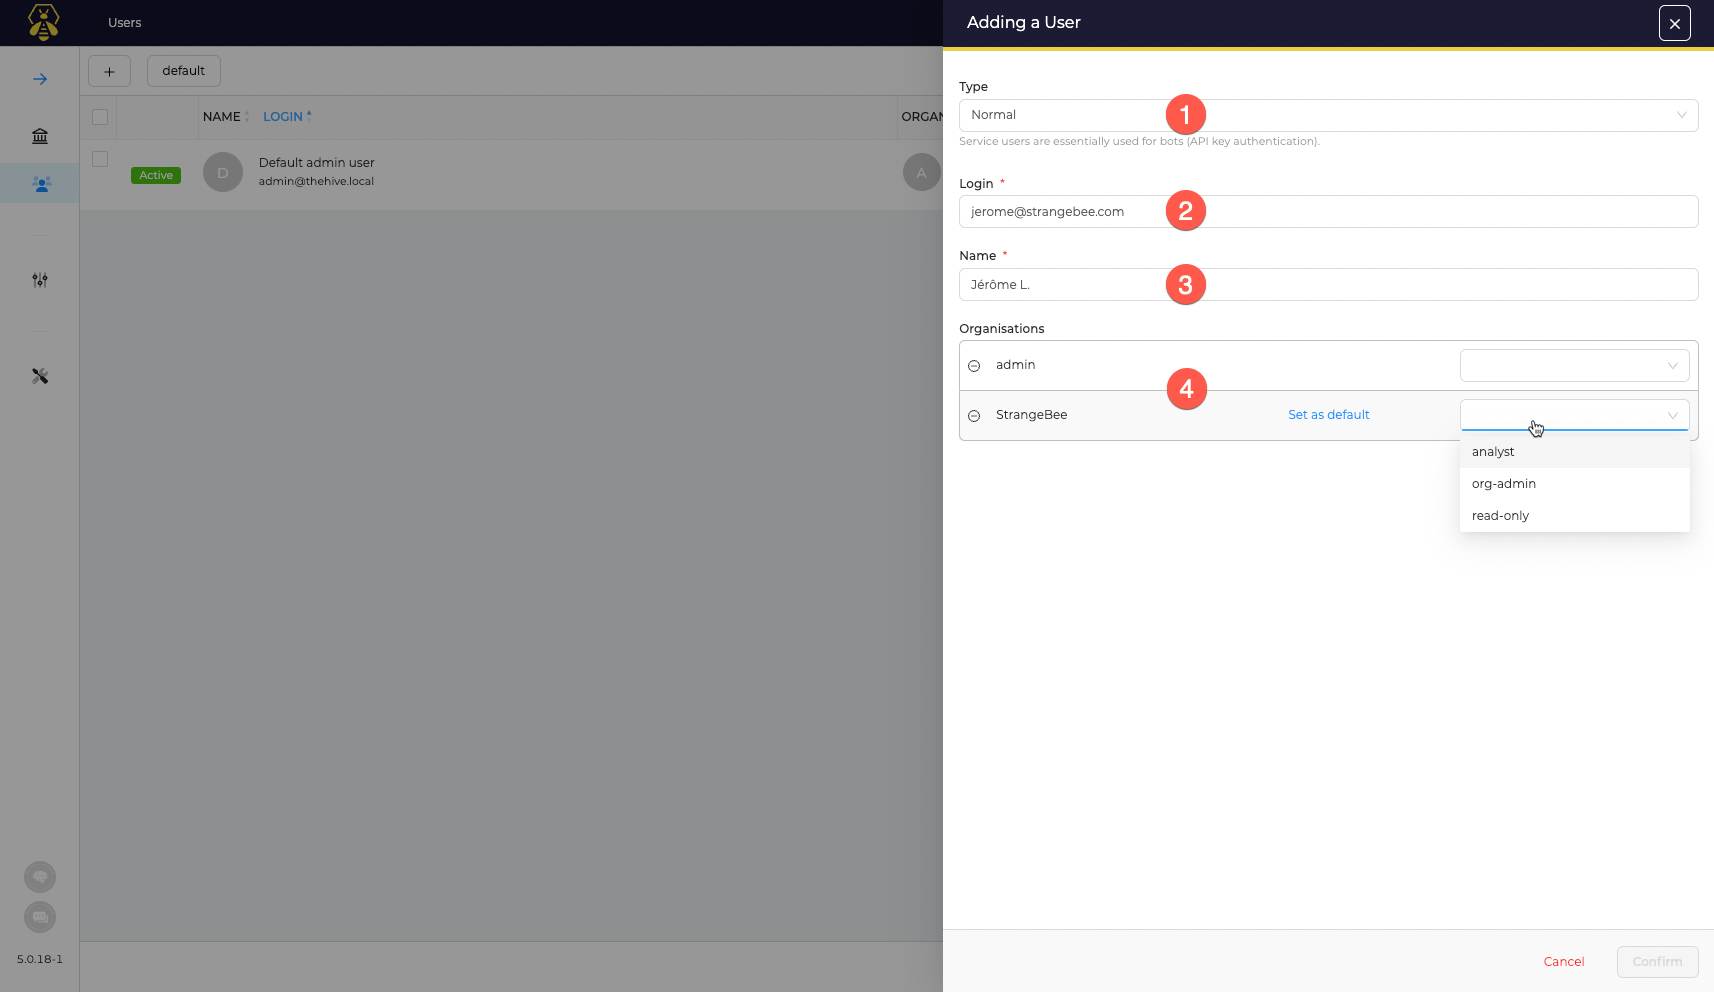
\includegraphics[width=0.8\textwidth]{accounts2.png}
    \caption{Add User}
    \label{fig:add}
\end{figure}

We can also edit an existing account by clicking on the \textbf{preview} button. \\

\subsection{Entities \& Permissions}
TheHive comes with a set of predefined profiles for Administrators and Organsations ; this set can be enriched with custom profiles you can create depending on your needs.\\
We can see this in Figure \ref{fig:entities}.
\begin{figure}[H]
    \centering
    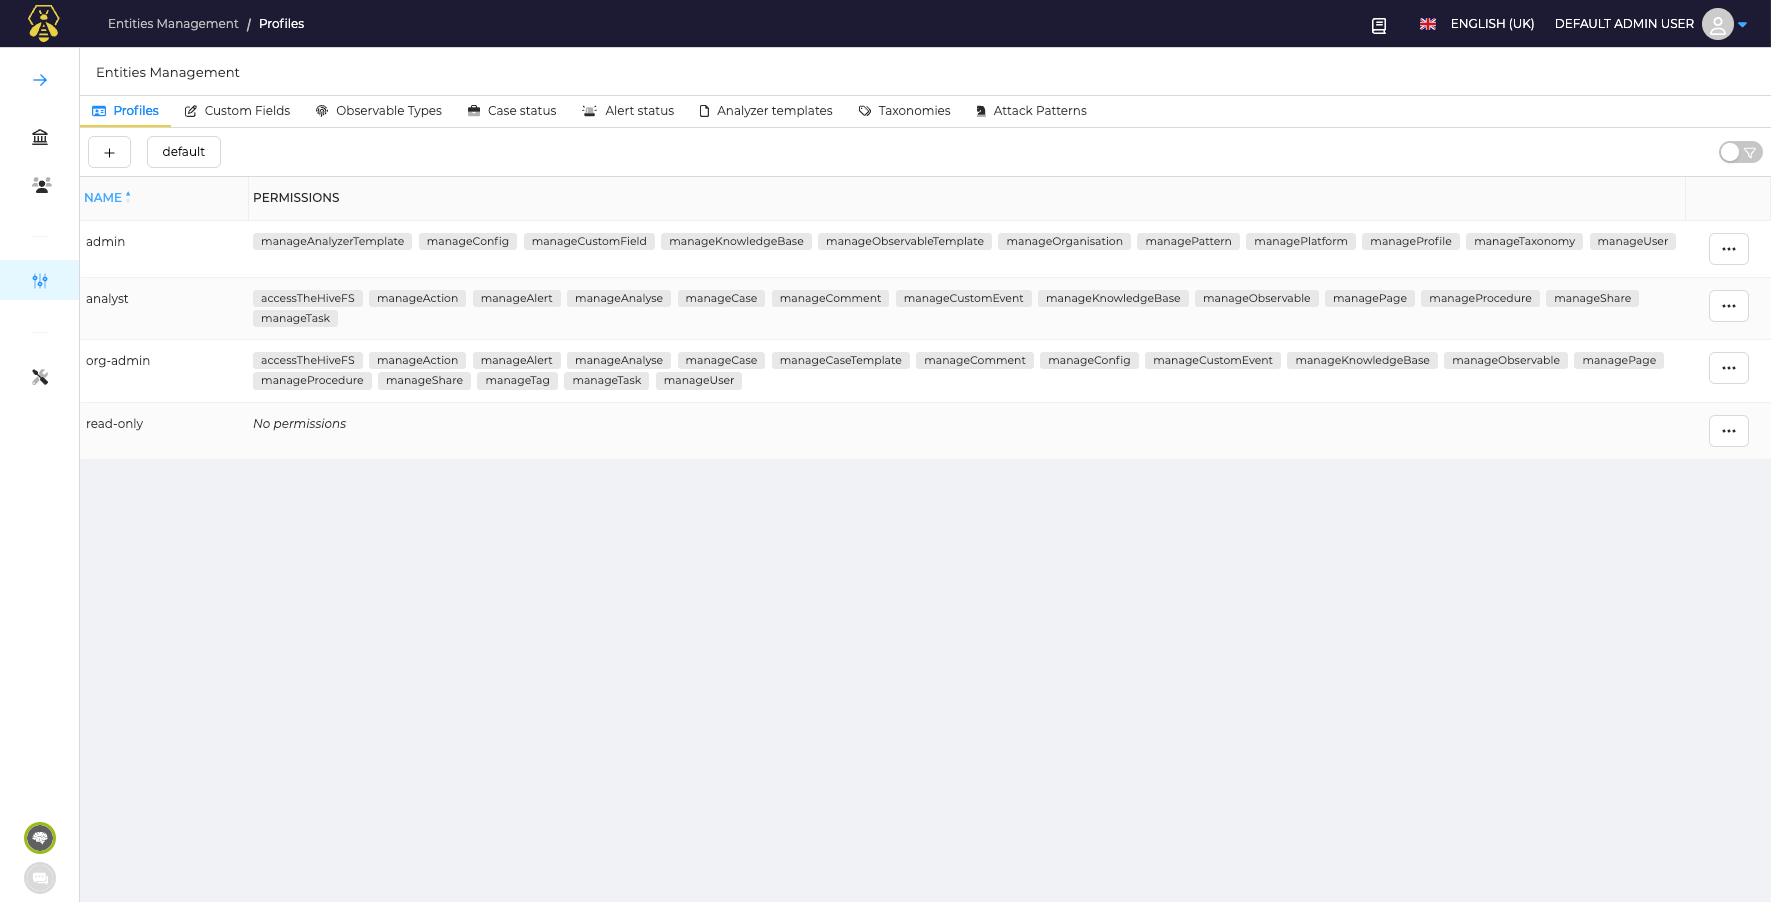
\includegraphics[width=0.8\textwidth]{entities.png}
    \caption{Entities avaliable}
    \label{fig:entities}
\end{figure}

Users are given Permissions by their roles. \\
Permissions are defined for each entity of the application.\\
The following entities are available:
\begin{itemize}
    \item admin
    \item analyst
    \item org-admin
    \item read-only
\end{itemize}

\subsection{Users Roles}
Now that we have created our users, we need to assign them roles.\\
We have the entities given in Figure \ref{fig:entities}. We can give roles according to our needs.\\
\begin{enumerate}
    \item \textbf{Admin}:
       \begin{itemize}
         \item \textbf{Description}: Administrators have full control over TheHive platform. They can create, modify, and delete accounts, organizations, and configurations. Administrators typically manage the overall settings and ensure the platform functions smoothly.
         \item \textbf{Privileges}:
         \begin{itemize}
           \item Full access to all features and functionalities.
           \item User and organization management.
           \item Configuration and system settings control.
           \item Incident case management.
         \end{itemize}
       \end{itemize}
    \item \textbf{Analyst}:
       \begin{itemize}
         \item \textbf{Description}: Analysts are standard users responsible for working on incident cases and investigations within TheHive. They have access to case management and analysis tools to investigate and respond to security incidents.
         \item \textbf{Privileges}:
         \begin{itemize}
           \item Access to incident case management.
           \item Ability to work on and update cases.
           \item Collaboration with other analysts.
           \item Limited access to system configurations.
         \end{itemize}
       \end{itemize}
  
    \item \textbf{Org-admin} (Organization Administrator):
       \begin{itemize}
         \item \textbf{Description}: Organization administrators have administrative privileges limited to a specific organization within TheHive. They can manage users, incidents, and configurations for their assigned organization.
         \item \textbf{Privileges}:
         \begin{itemize}
           \item User management within their organization.
           \item Incident case management within their organization.
           \item Limited access to system-wide configurations.
           \item May not have access to other organizations' data.
         \end{itemize}
       \end{itemize}
  
    \item \textbf{Read-only}:
       \begin{itemize}
         \item \textbf{Description}: Read-only users have limited access and are primarily meant for users who need to view incident cases and data without making changes or updates. They can review and gather information but cannot modify cases.
         \item \textbf{Privileges}:
         \begin{itemize}
           \item View-only access to incident cases and data.
           \item Cannot modify or update cases.
           \item Limited interaction with the platform.
         \end{itemize}
       \end{itemize}
  \end{enumerate}

  \subsection{Observables types, cases and alert status}
TheHive allows administrators to create multiple observables types within the tool. Each observable type can have its own set of attributes. This allows for better separation of duties and responsibilities between different teams within an organization, such as a SOC team and a CSIRT team.\\
To create a new observable type, follow these steps: \\
\begin{enumerate}
\item  Click on the \textbf{Add an Observable Type} button.
\item  Edit the required fields in the drawer:
   \begin{itemize}
        \item Name: Name of the new Observable Type.
        \item Description: Description for the new Observable Type.
        \item Attribute: Attribute for the new Observable Type.
    \end{itemize}
\item Click \textbf{Confirm} to create the observable type.
\end{enumerate}

We can see this in Figure \ref{fig:observables}.
\begin{figure}[H]
    \centering
    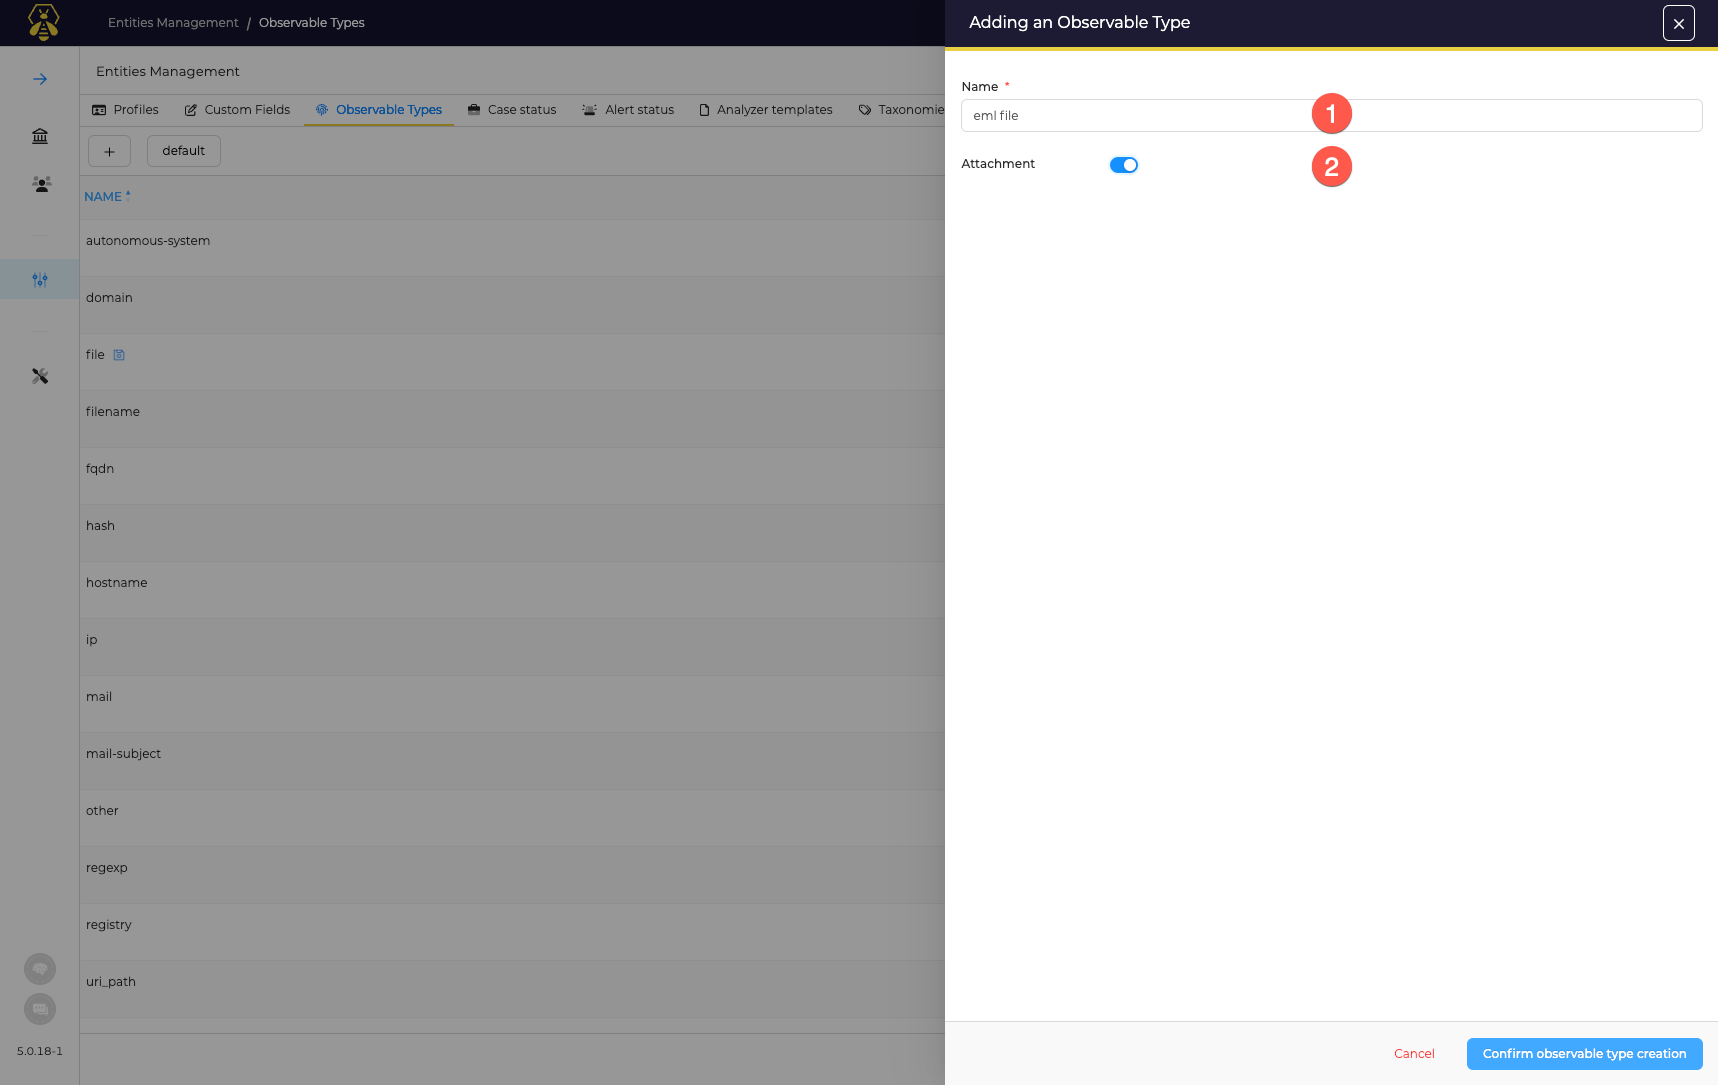
\includegraphics[width=0.8\textwidth]{observable-types.png}
    \caption{Create Observables}
    \label{fig:observables}
\end{figure}

Admin can also add new status for cases and alerts.\\
To define a status, you need to specify the following:

\begin{enumerate}
  \item \textbf{Stage}: Choose the stage of the new status.
  \item \textbf{Value}: Choose a name for the new status.
  \item \textbf{Color}: Choose a color for users to quickly identify the status in the application.
\end{enumerate}

\subsection*{Example:}

\begin{itemize}
  \item \textbf{Stage}: Investigation
  \item \textbf{Value}: In Progress
  \item \textbf{Color}: \textcolor{blue}{Blue}
\end{itemize}

In this example, a status "In Progress" is defined for the "Investigation" stage with a blue color to help users identify it in the application.


\section{User side}
TheHive has a web-based user interface that allows users to access the tool from any computer with an Internet connection. Users can create incidents, add comments and attachments to them, assign tasks to other users, and close incidents when they are resolved. They can also search for incidents based on various criteria such as their status, severity level, or creation date. Users can also create reports based on the data stored in the tool's database.
list of features:
\begin{itemize}
\item Incident management
\item Case management
\item Task management
\item Report management
\item Dashboard management
\item Integration with other tools
\end{itemize}

\subsubsection{Templetes}
As a org-admin, one can create templates for incidents.\\
One can create templetes for cases, pages and reports.\\
We will see how to create templetes for cases.\\
First, let's see the lists of case templetes.\\
Access to the list by opening the Organisation menu, then the Templates tab, and the Cases tab.

We can see this in Figure \ref{fig:templetes}.
\begin{figure}[h!]
    \centering
    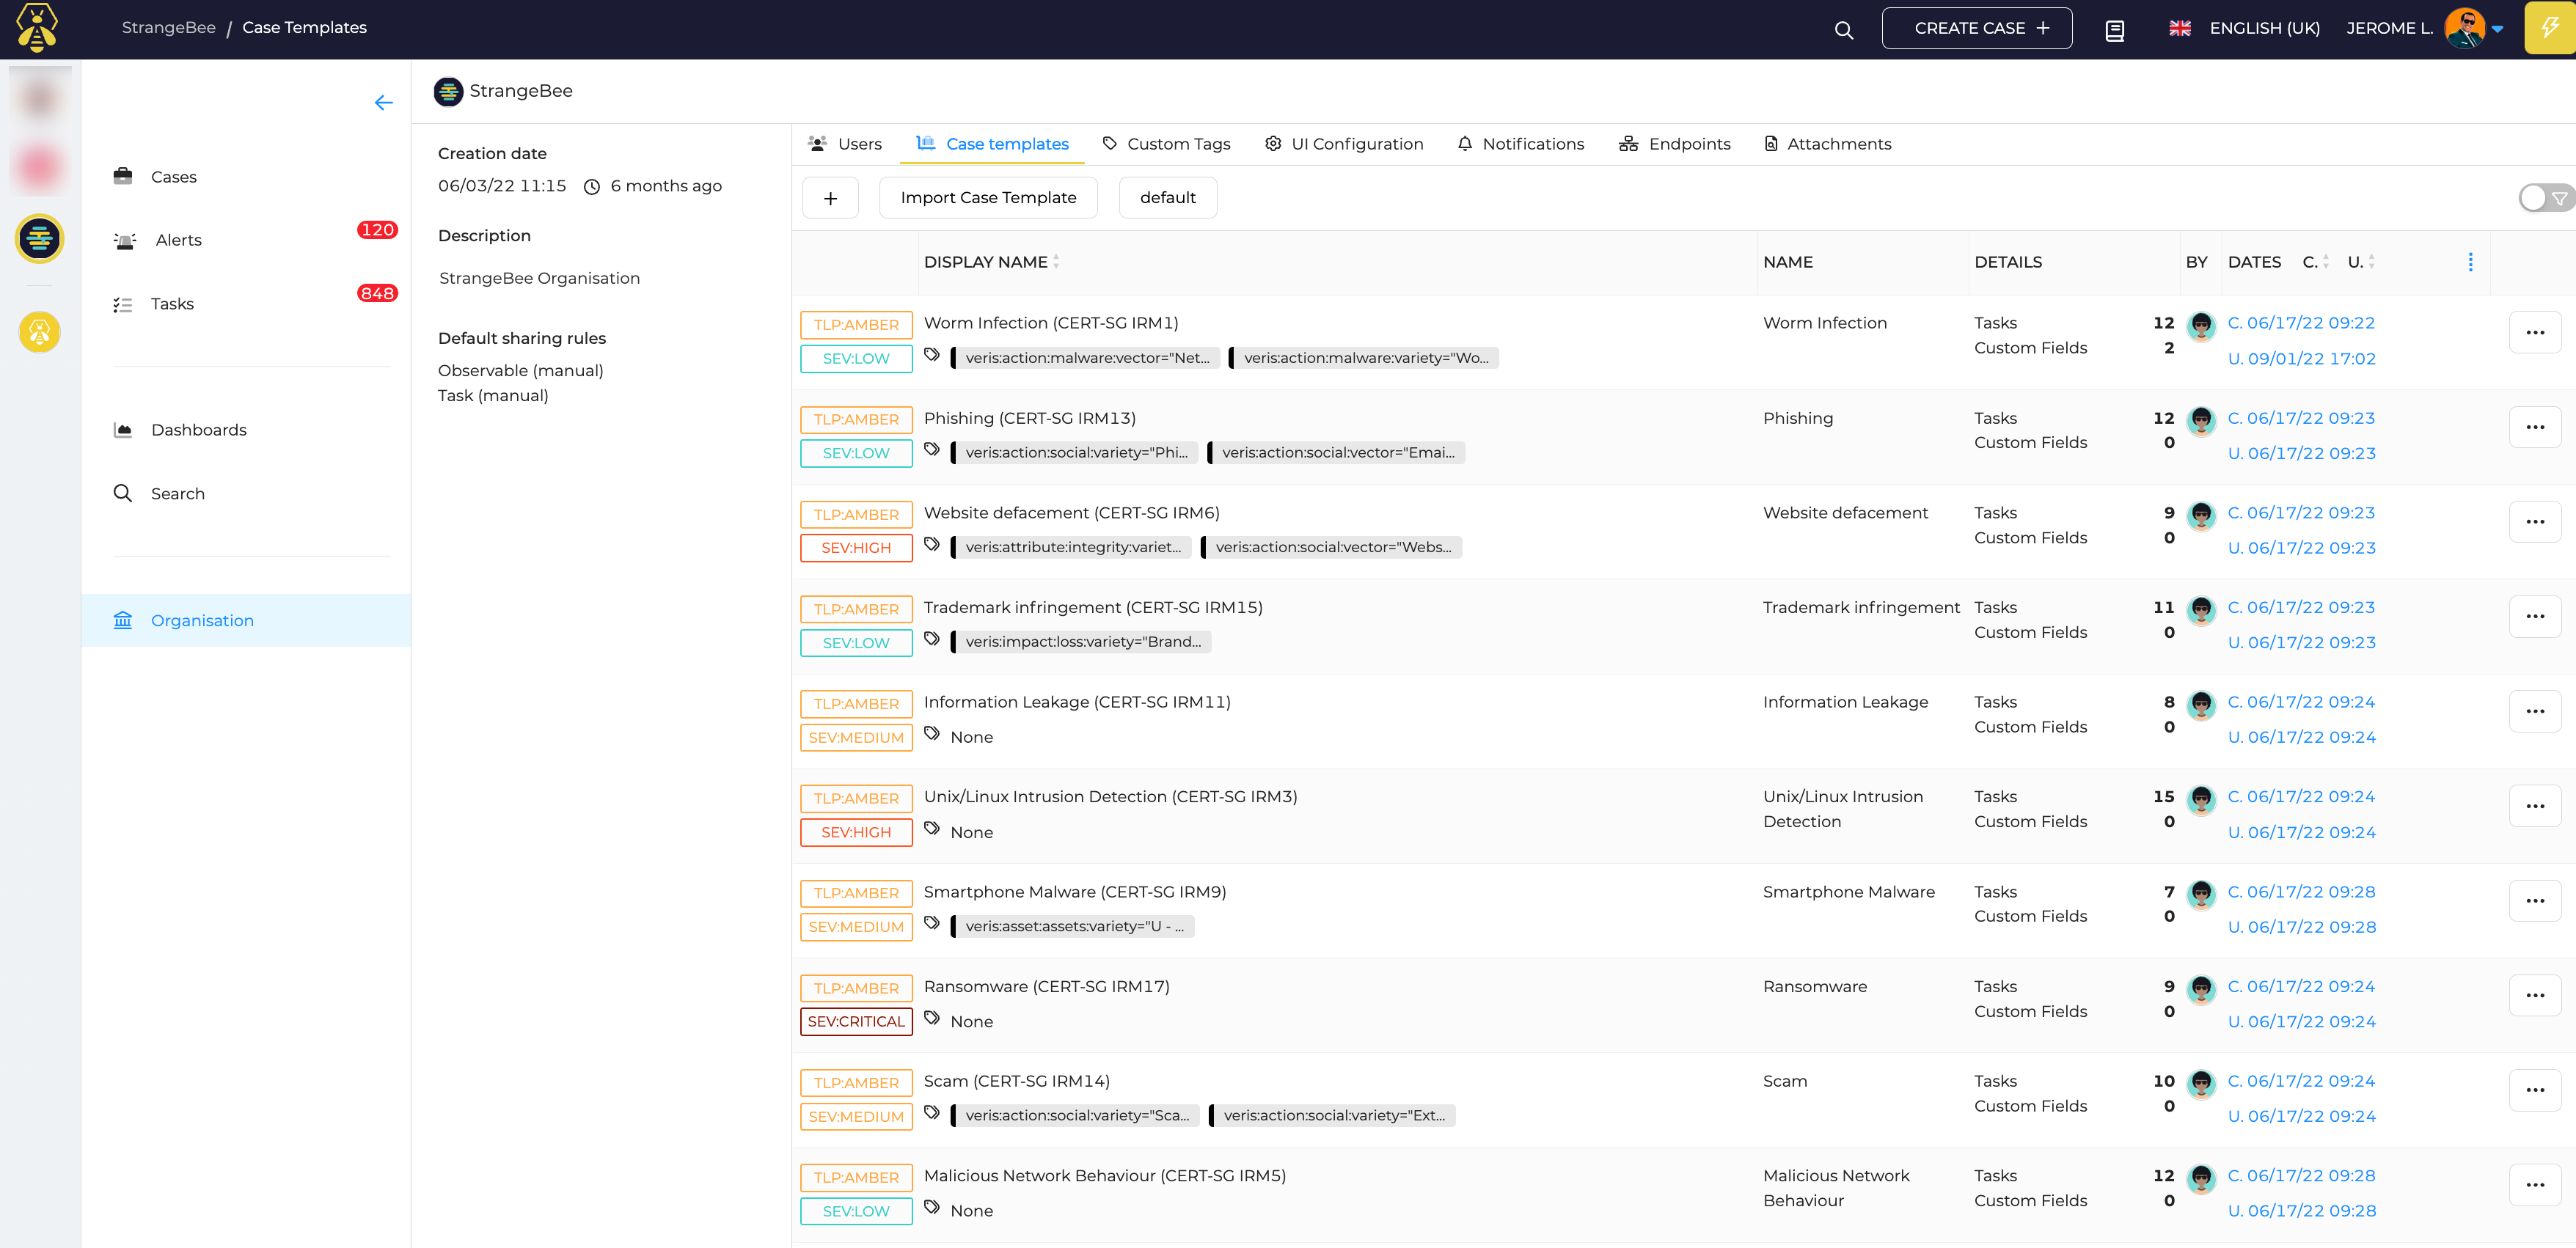
\includegraphics[width=0.8\textwidth]{organisation-case-templates1.png}
    \caption{List of Case templates}
    \label{fig:templetes}
\end{figure}

Click the plus button to create a new Case template.

We can see this in Figure \ref{fig:new}.
\begin{figure}[h!]
    \centering
    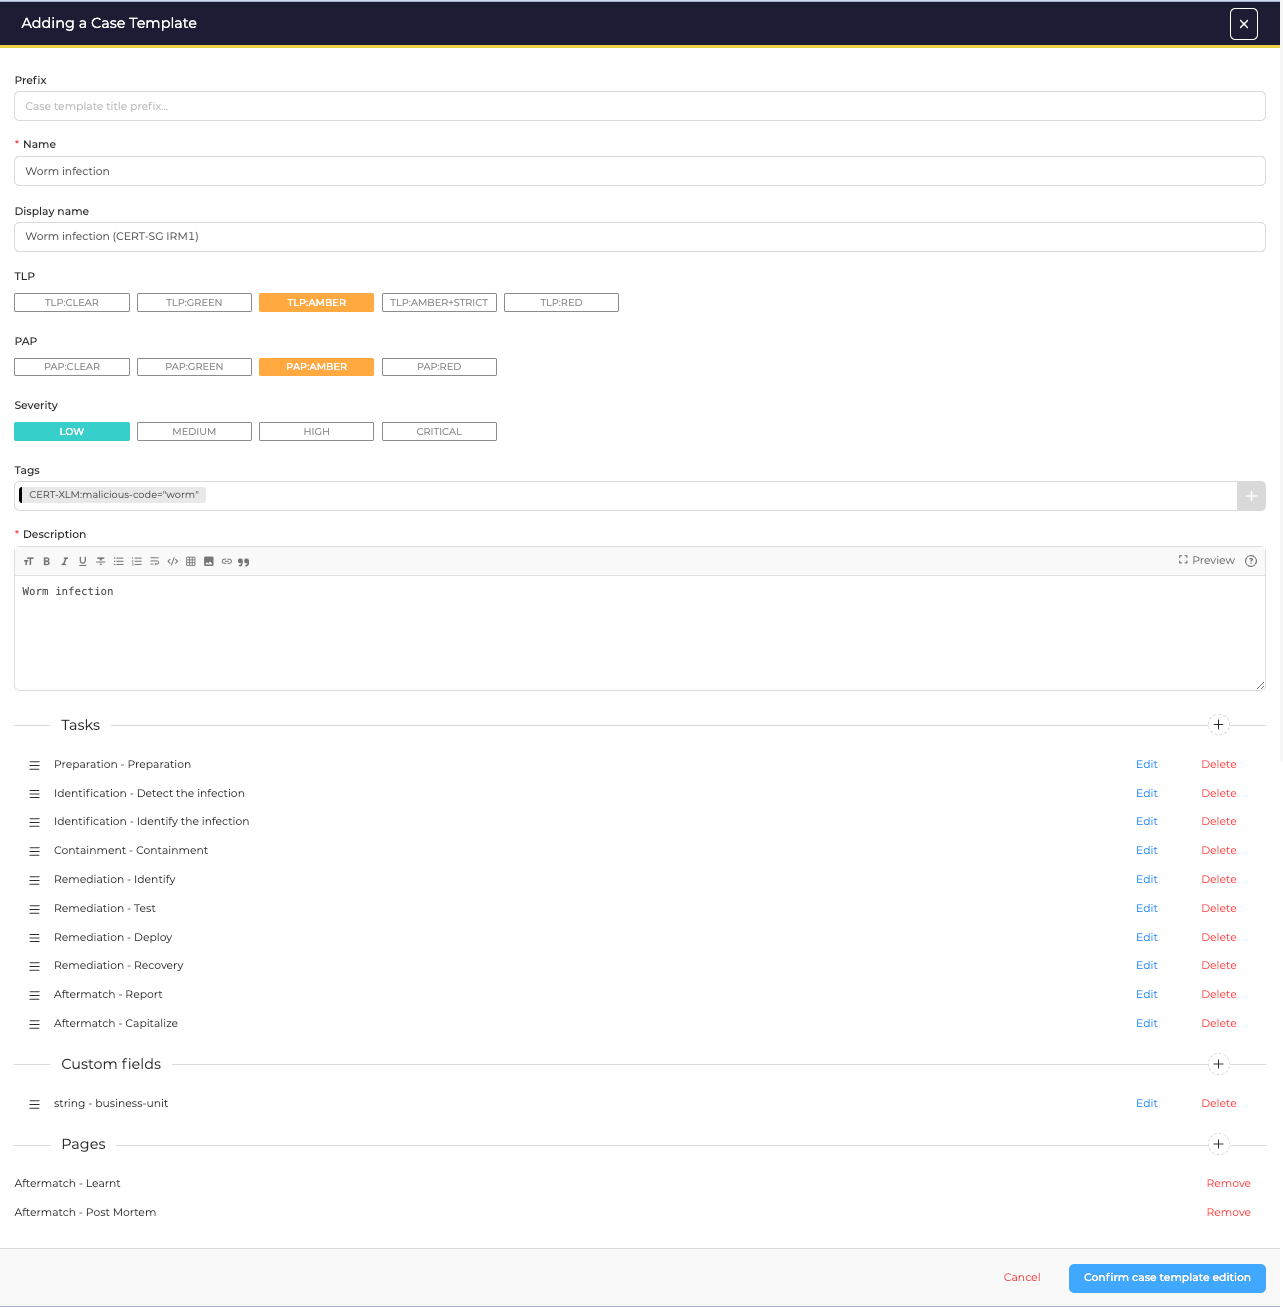
\includegraphics[width=0.8\textwidth]{organisation-case-templates2.png}
    \caption{New Case template}
    \label{fig:new}
\end{figure}

\subsection*{Configuration parameters:}
When creating a Case template, you can configure the following parameters:

\begin{enumerate}
  \item \textbf{Prefix}: String that will be prepended to the title of a Case when created with this template.
  \item \textbf{Name}: Name of the Case template. Used to identify the Case template with the API.
  \item \textbf{Display Name}: Name of the Case template displayed in the UI.
  \item \textbf{TLP}: Default TLP (Traffic Light Protocol) of the Case when created with this template.
  \item \textbf{PAP}: Default PAP (Perceived Attribution Program) of the Case when created with this template.
  \item \textbf{Severity}: Default Severity of the Case when created with this template.
  \item \textbf{Tags}: List of tags that will be added to the Cases created with this template.
  \item \textbf{Description}: Default description of Cases created with this template if not modified.
  \item \textbf{Tasks}: Add tasks to the templates. They will be automatically added to the Case when created with this template.
  \item \textbf{Custom Fields}: Add Custom fields to the template. Default values can be set for Custom fields as well.
  \item \textbf{Pages}: Add pages template to the template. They will be automatically added to the Case when created with this template.
\end{enumerate}

\subsection*{Import/Export}

\subsection*{Export a Case Template}

To export a Case template, follow these steps:

\begin{enumerate}
  \item Click on the option icon (usually represented as three dots or a gear icon).
  \item Select "Export case template" from the menu.
\end{enumerate}

The Case template will be exported and saved as a JSON file. //

We can see this in Figure \ref{fig:export}.
\begin{figure}[h!]
    \centering
    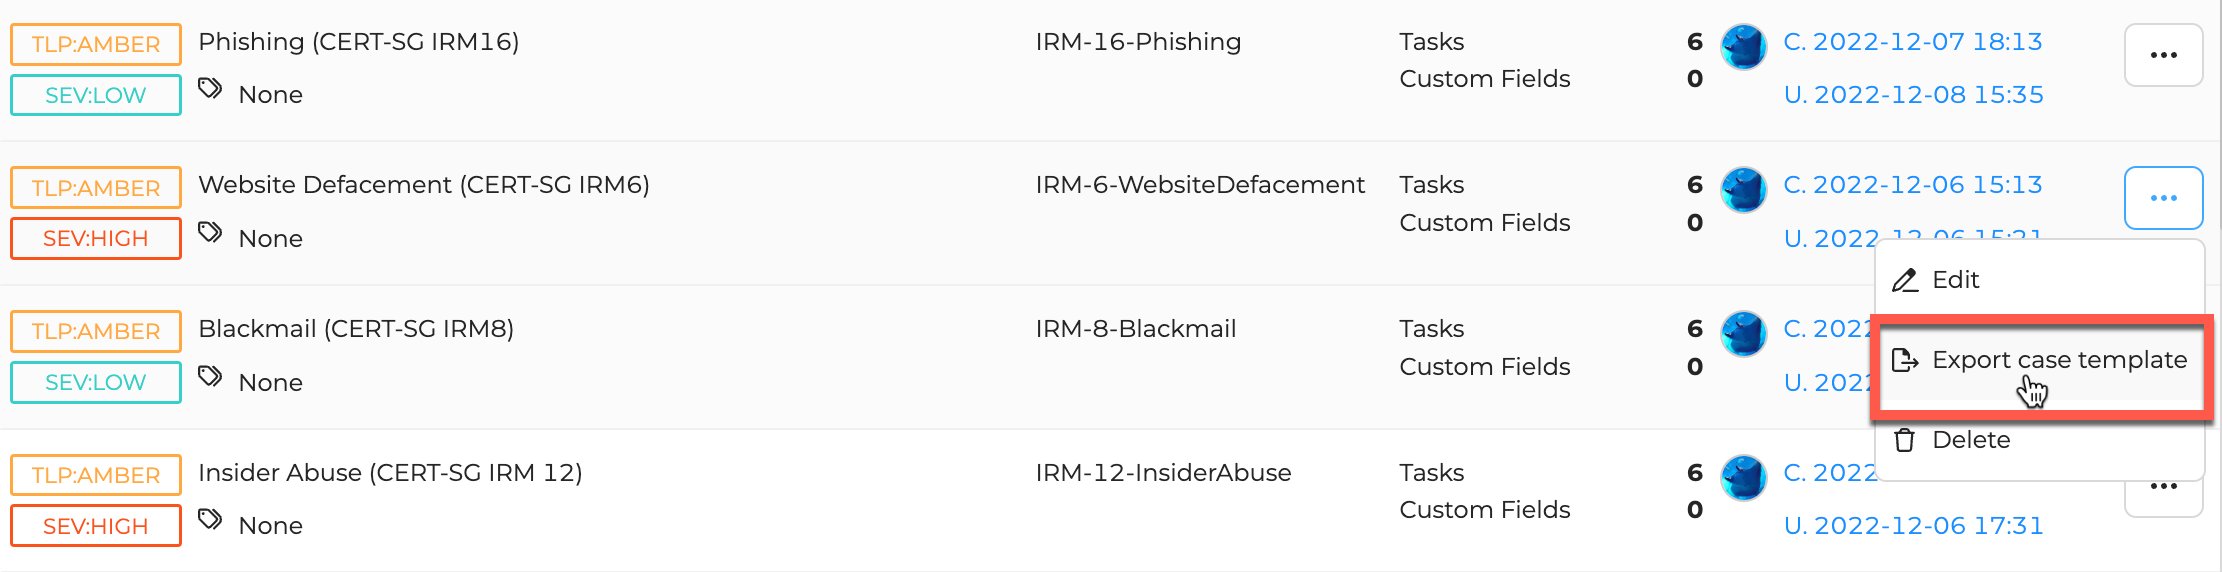
\includegraphics[width=0.8\textwidth]{organisation-case-templates-3.png}
    \caption{Export Case template}
    \label{fig:export}
\end{figure}

\subsection*{Import a Case Template}

To import a Case template, follow these steps:

\begin{enumerate}
  \item Click on the \textbf{Add a Case Template} button.
  \item Select the JSON file containing the Case template.
  \item Click \textbf{Confirm} to import the Case template.
\end{enumerate}

We can see this in Figure \ref{fig:import}.
\begin{figure}[H]
    \centering
    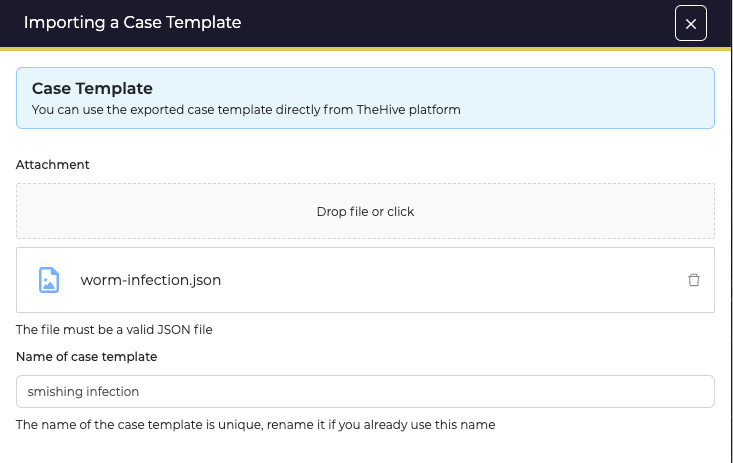
\includegraphics[width=0.8\textwidth]{organisastion-case-templates-4.png}
    \caption{Import Case template}
    \label{fig:import}
\end{figure}

\subsection{Alerts}

Alerts provide timely information about current security issues, vulnerabilities, and exploits.

\subsubsection{View Alert Details}

To view the details of an alert, follow these steps:

\begin{enumerate}
  \item Click on the \textbf{Alerts} button in the left menu.
  \item Click on the alert you want to view.
\end{enumerate}

The Alerts page displays various tabs that have more details about alerts such general tab, observables, TTPs, similar cases, similar alerts, responders tab.

We can see this in Figure \ref{fig:alert}.

\begin{figure}[H]
    \centering
    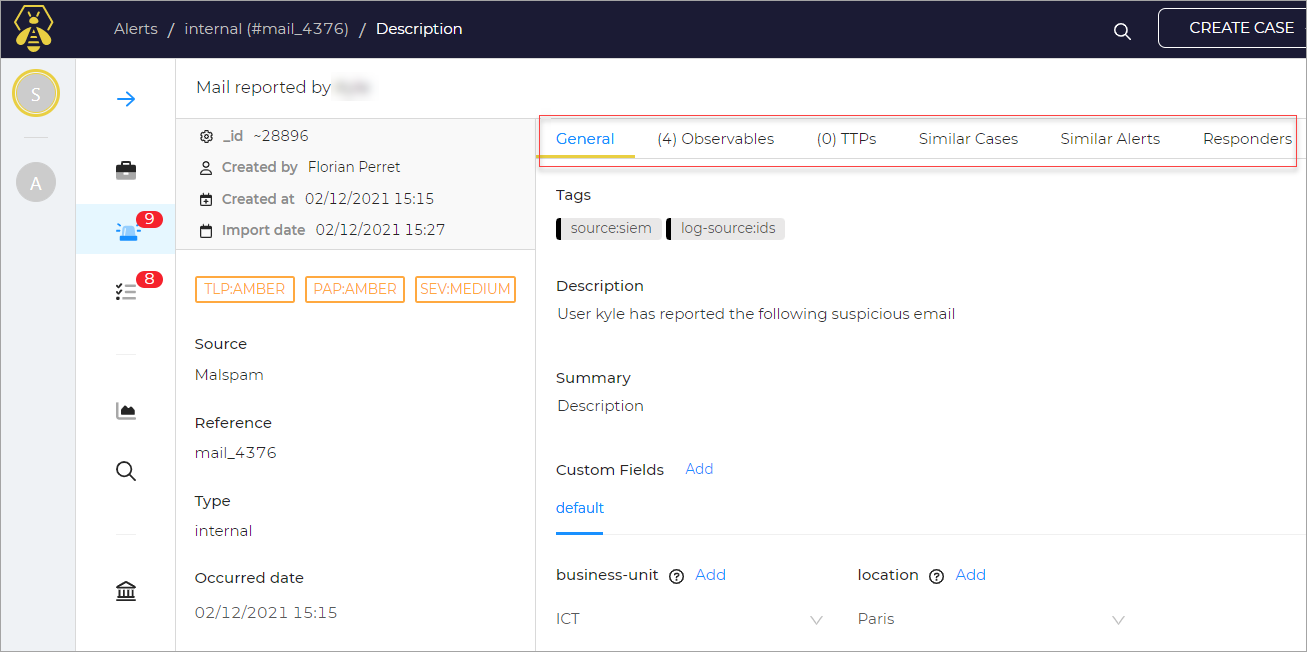
\includegraphics[width=0.8\textwidth]{alerts-menu-list.png}
    \caption{Alerts}
    \label{fig:alert}
\end{figure}

\subsubsection{Create a Case from an Alert}

On the main page where all the alerts are listed, there are various alerts. Some are new, some are imported. New case from selection option is available only for new alerts from the list.

We can see this in Figure \ref{fig:case}.
\begin{figure}[H]
    \centering
    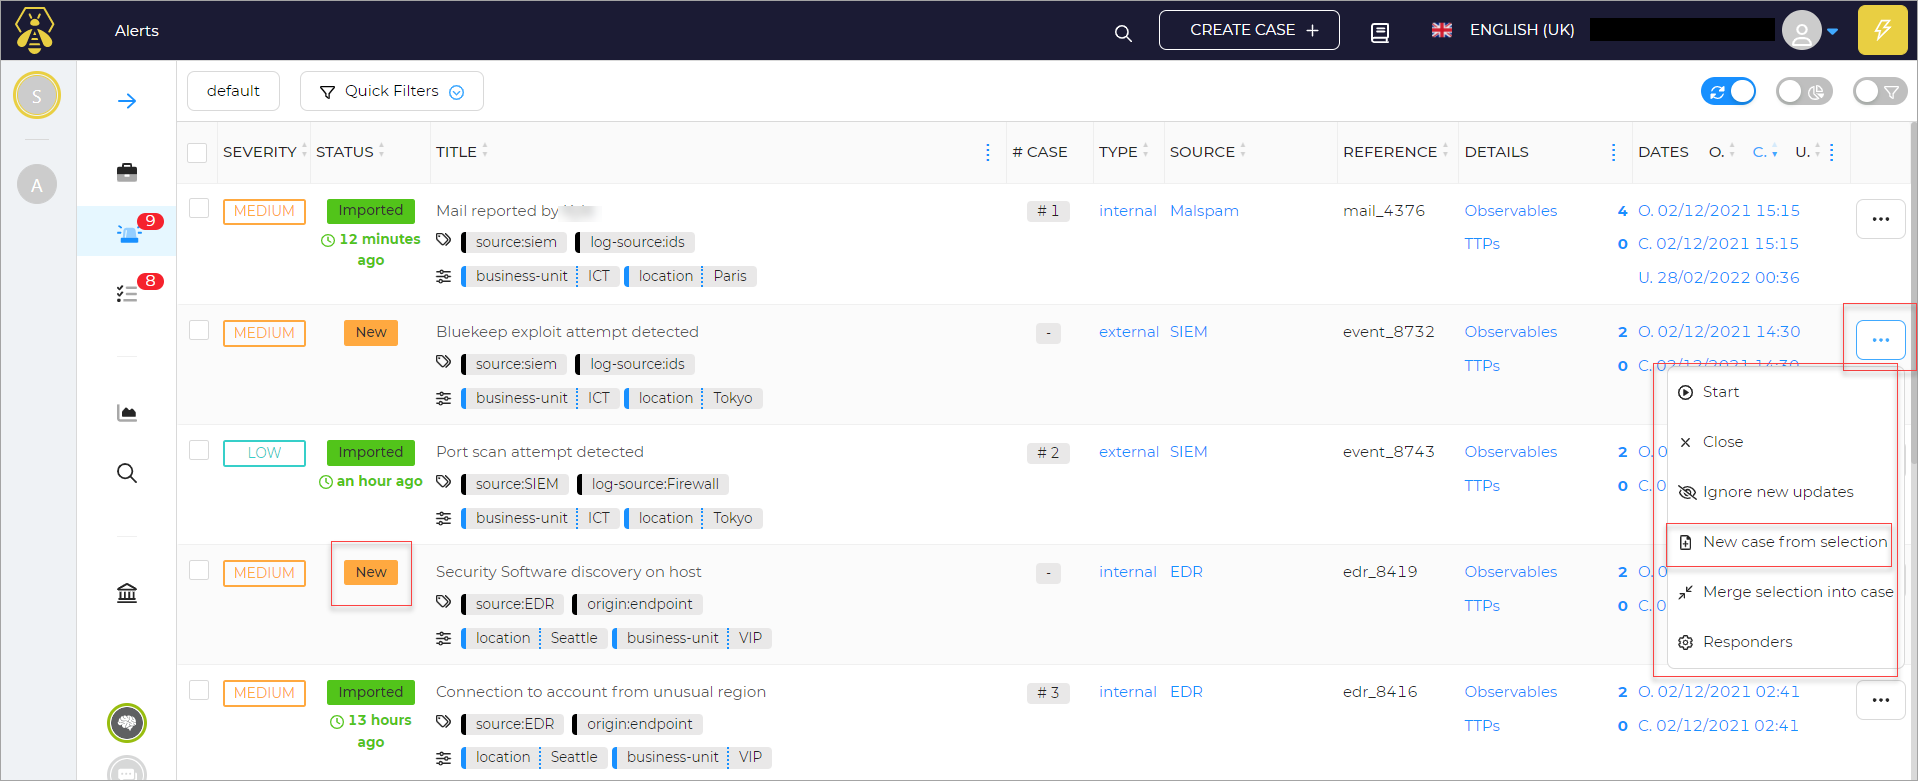
\includegraphics[width=0.8\textwidth]{alerts-actions1.png}
    \caption{Create Case from Alert}
    \label{fig:case}
\end{figure}

To add a new case from a selection, follow these steps:

\begin{enumerate}
  \item Go to the alert details page.
  \item Select the alert for which you want to add a new case.
  \item Click on the "New Case from Selection" option.
  \item A new window will open, allowing you to create a new case based on your selection.
\end{enumerate}

We can see this in Figure \ref{fig:newcase}.
\begin{figure}[H]
    \centering
    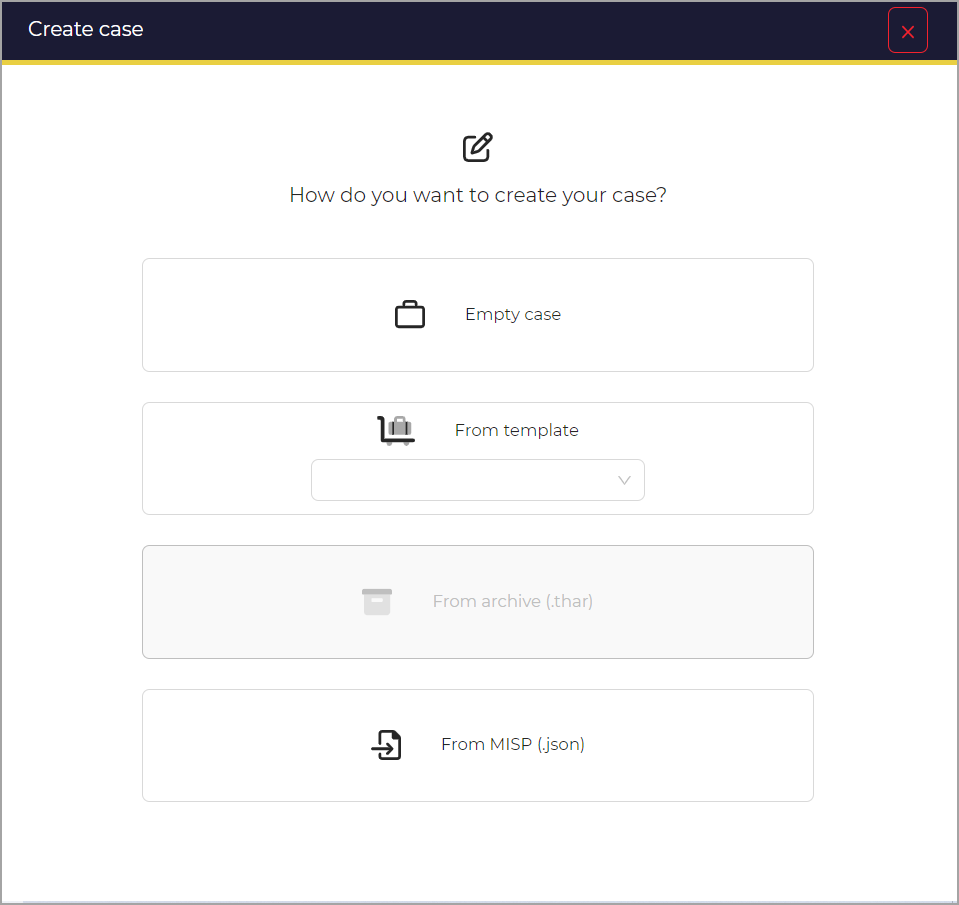
\includegraphics[width=0.8\textwidth]{alerts2.png}
    \caption{New Case from Alert}
    \label{fig:newcase}
\end{figure}

By selecting empty case  or case template, a new case will be created with the alert's observables and TTPs.\\



\subsection{Cases}

\begin{compactitem}
    \item A case provides information on suspicious activity in the environment. It provides information on the security incidents, observables, alerts, and affected users. Security analysts can conduct specific analysis based on cases to assess the possibilities of threats.
    \item Cases can be created from various sources. Each security case consists of a title, tags, task rules, obsevable rules a description of case details, and all the details related to the case that help in building an argument for identifying and dealing with particular threats.
\end{compactitem}

\subsubsection*{Create a Case}

To create new cases using templates, follow these steps:

\begin{enumerate}
  \item Click on "Create Case +" located in the header.
\end{enumerate}

\begin{figure}[H]
    \centering
    
\includegraphics[width=0.8\textwidth]{case1.png}
    \caption{Create Case}
    \label{fig:createcase}
\end{figure}

One can create case from:
\begin{itemize}
    \item Empty Case
    \item Case Template
    \item Archive
    \item From MISP (.json)

\end{itemize}

We can see this in Figure \ref{fig:casefrom}.
\begin{figure}[H]
    \centering
    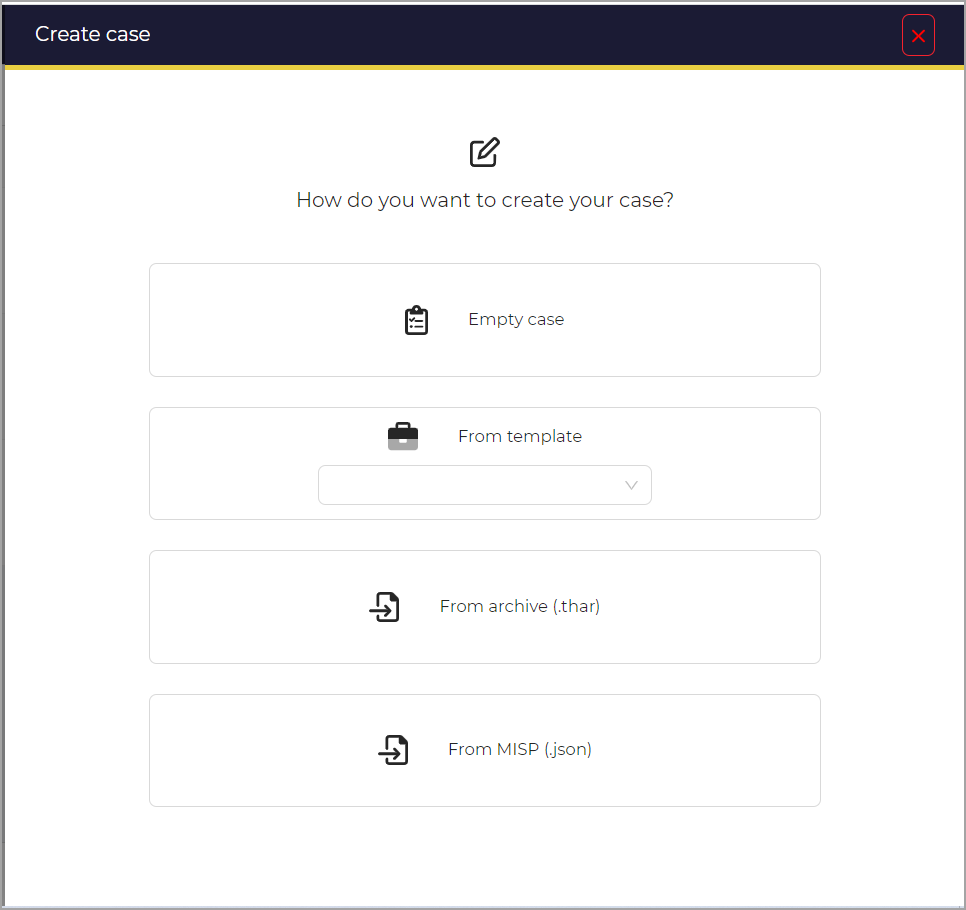
\includegraphics[width=0.8\textwidth]{case2.png}
    \caption{Create Case from}
    \label{fig:casefrom}
\end{figure}

We will create case from empty case.\\

\subsubsection*{Creating a New Case from an Empty Case}

To create a new case from an empty case, follow these steps:

\begin{enumerate}
  \item Enter the case title in the "Title" field.
  \item Select a date from the "Date" field.
  \item Select the severity level (Low/Medium/High/Critical).
  \item Select the TLP (Traffic Light Protocol) level (White/Green/Amber/Red).
  \item Select the PAP (Perceived Attribution Program) level (White/Green/Amber/Red).
  \item Click the "+" button to add tags (refer to "Add Tags").
  \item Enter the case description in the "Description" field.
  \item Choose a Task rule from the list (manual/existingOnly/upcomingOnly/all).
  \item Choose an Observable rule from the list (manual/existingOnly/upcomingOnly/all).
  \item Add tasks (refer to "Add Tasks").
  \item Add custom fields (refer to "Add Custom Field Values").
  \item Click the "Confirm case creation" button to create the case.
\end{enumerate}

You have successfully created a new case from an empty case.

We can see this in Figure \ref{fig:emptycase}.
\begin{figure}[H]
    \centering
    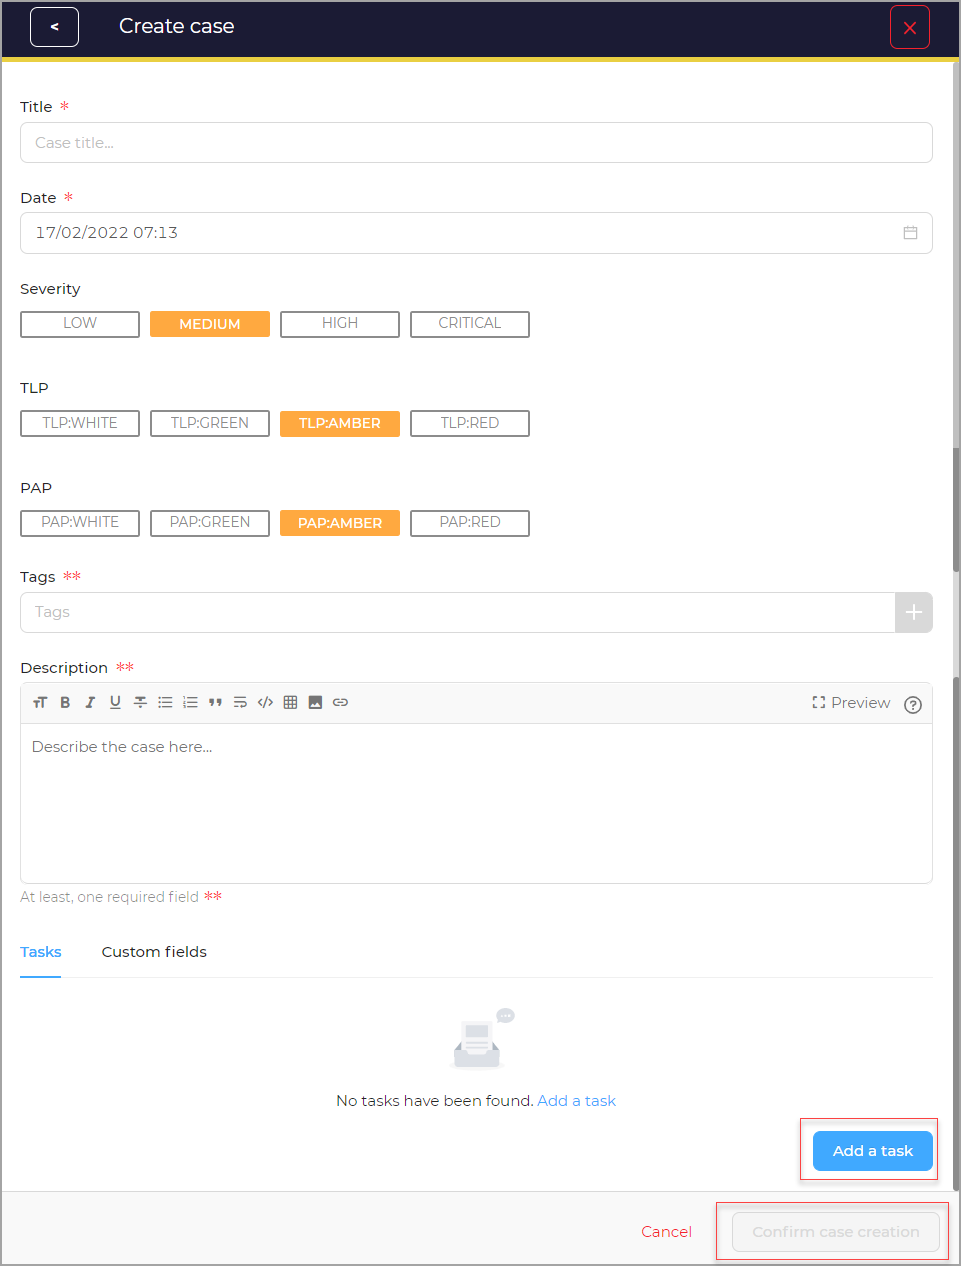
\includegraphics[width=0.8\textwidth]{case3.png}
    \caption{Empty Case}
    \label{fig:emptycase}
\end{figure}

\subsection{Tasks}
Task details, require action from its users. Task details page displays a list of tasks. When navigating through the Task list, you can easily see and determine which Task needs an action.

\subsubsection*{To view task details}
One can view task details by clicking on the tasks in the list.\\

\begin{figure}[H]
    \centering
    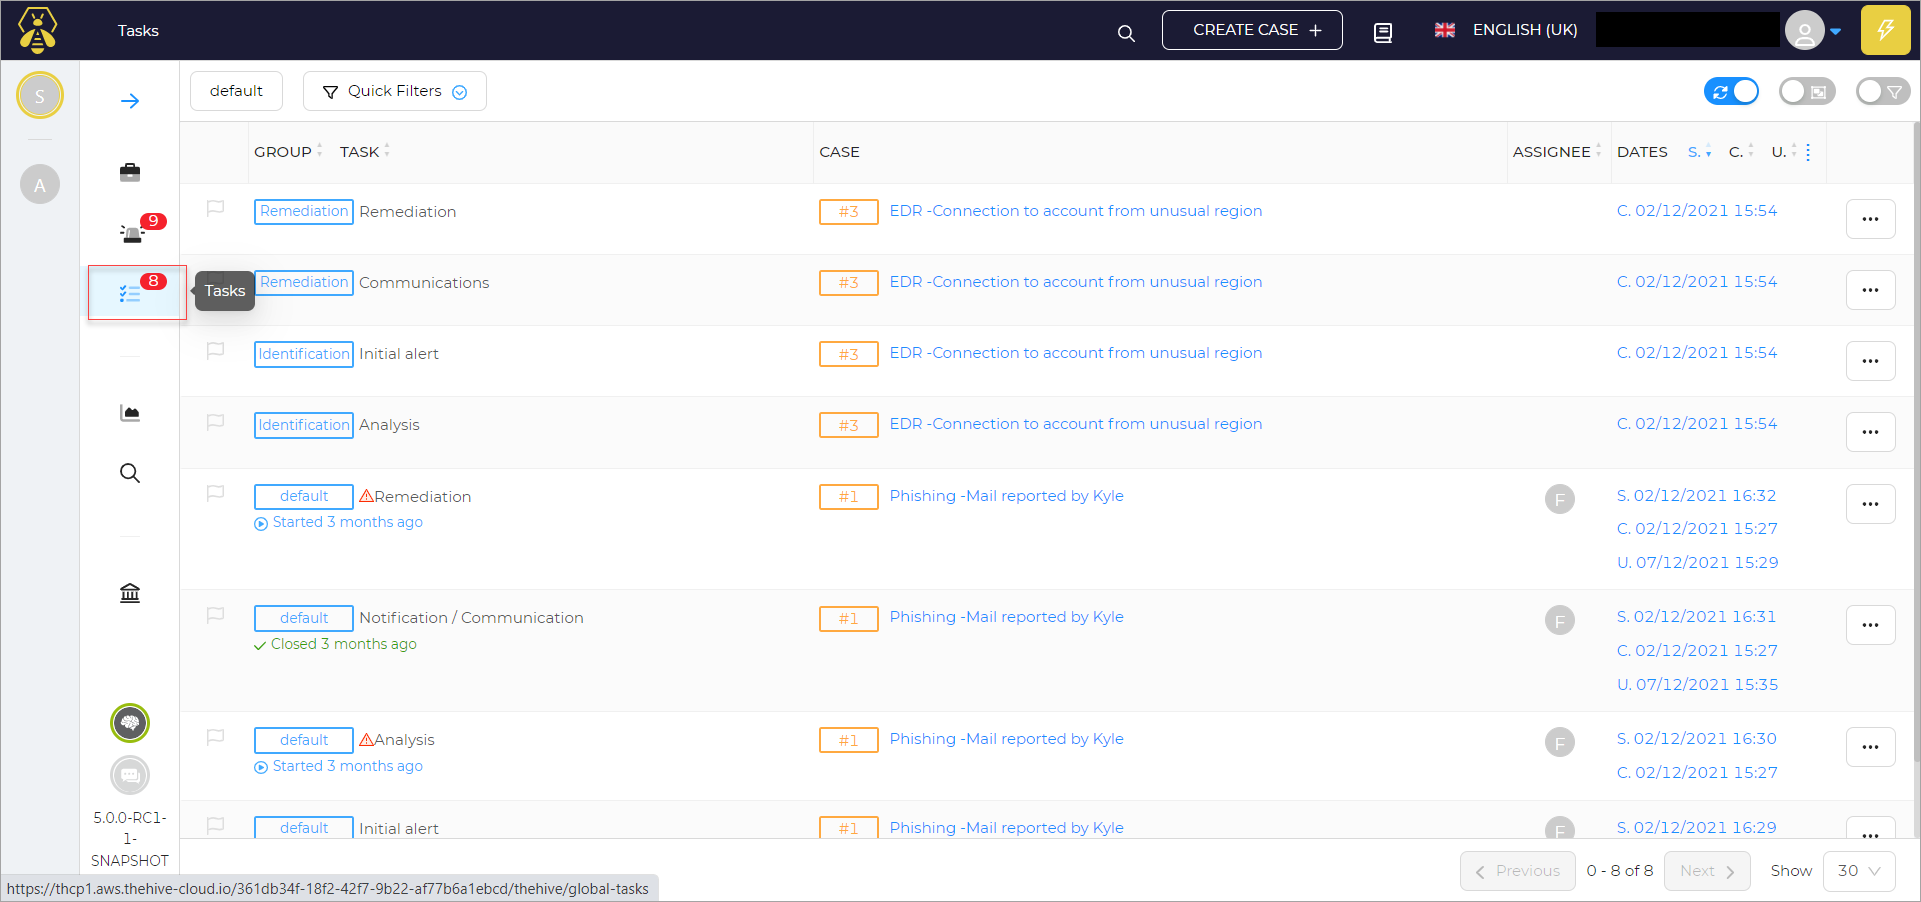
\includegraphics[width=0.8\textwidth]{task1.png}
    \caption{Task}
    \label{fig:task}
\end{figure}

The details are displayed

\begin{figure}[H]
    \centering
    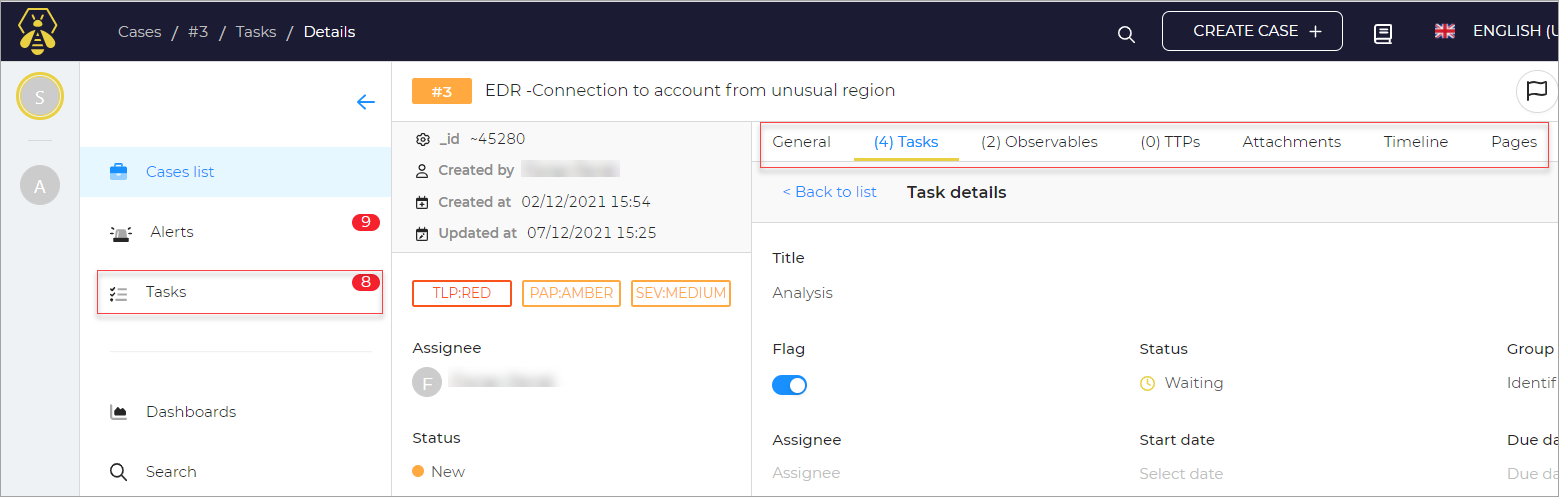
\includegraphics[width=0.8\textwidth]{task2.png}
    \caption{Task Details}
    \label{fig:taskdetails}
\end{figure}

\subsubsection*{Task creation}
After creating a case, one can add tasks to the case and assigning each task to one or many users so that they can work on it.\\
To add a task to a case, follow these steps:

\begin{enumerate}
  \item Click on the "Add a Task" button which is shown in figure \ref{fig:taskcreate}.
\end{enumerate}

\begin{figure}[H]
    \centering
    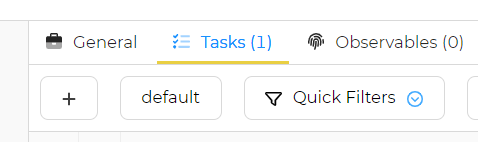
\includegraphics[width=0.8\textwidth]{addTask1.png}
    \caption{Task Create}
    \label{fig:taskcreate}
\end{figure}

After clicking, one can see the following window represented in figure \ref{fig:taskcreate1}.

\begin{figure}[H]
    \centering
    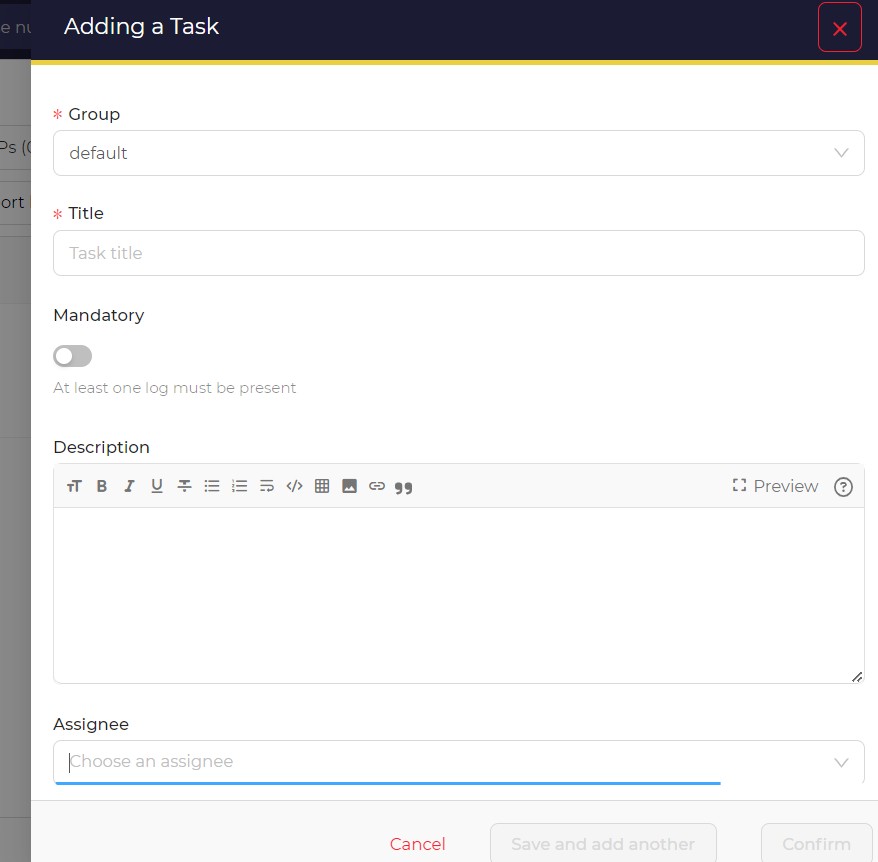
\includegraphics[width=0.8\textwidth]{addTask2.png}
    \caption{Task Create}
    \label{fig:taskcreate1}
\end{figure}

By filling up necessary fields, one can create a task and assign it to a user by selecting assignee from the list.\\

\subsubsection*{Configure case details}

Every case has three important elements the TLP, PAP and Severity. TLP defines the confidentiality of information. PAP is the level of exposure of information to the outsde world and Severity implies the severity of information.

\subsubsection*{Configuring TLP (Confidentiality of Information)}

To configure TLP (Traffic Light Protocol) for the confidentiality of information, follow these steps:

\begin{enumerate}
  \item Select TLP from the list of options, which includes White, Green, Amber, and Red.
\end{enumerate}

Choose the appropriate TLP level based on the confidentiality requirements of the information.

\begin{figure}[H]
    \centering
    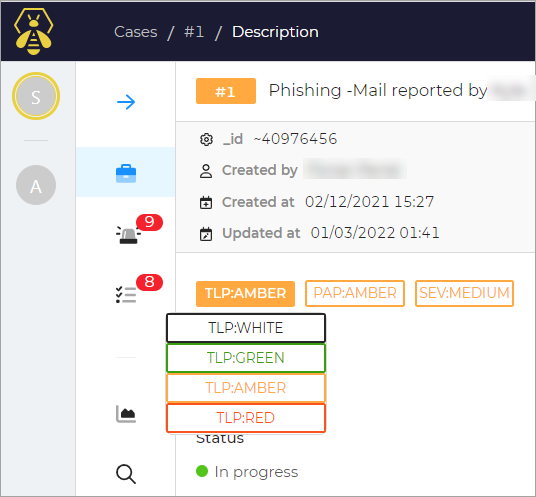
\includegraphics[width=0.8\textwidth]{configure1.png}
    \caption{TLP}
    \label{fig:tlp}
\end{figure}

\subsubsection*{Configuring PAP (Level of exposure of information)}

To configure PAP (Perceived Attribution Program) for the level of exposure of information, follow these steps:

\begin{enumerate}
  \item Select PAP from the list of options, which includes White, Green, Amber, and Red.
\end{enumerate}

Choose the appropriate PAP level based on the exposure requirements of the information.

\begin{figure}[H]
    \centering
    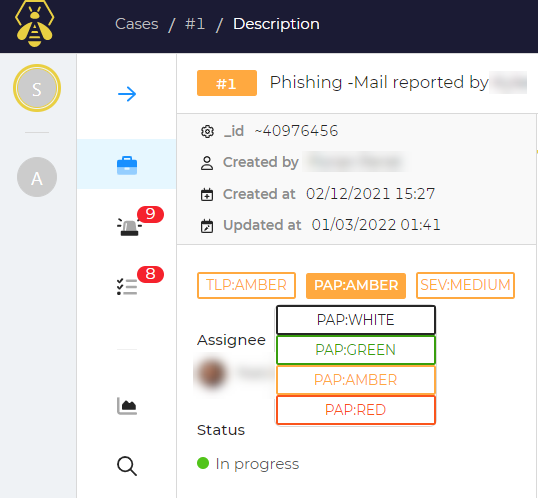
\includegraphics[width=0.8\textwidth]{configure2.png}
    \caption{PAP}
    \label{fig:pap}
\end{figure}

\subsubsection*{Configuring Severity (Severity of Information)}

To configure Severity for the severity of information, follow these steps:

\begin{enumerate}
  \item Select Severity from the list of options, which includes Low, Medium, High, and Critical.
\end{enumerate}

Choose the appropriate Severity level based on the severity requirements of the information.

\begin{figure}[H]
    \centering
    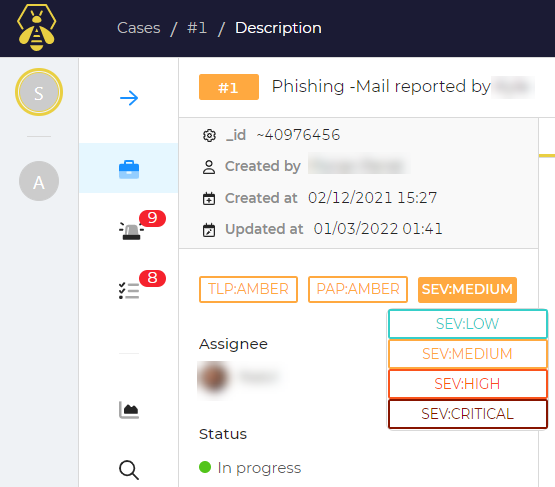
\includegraphics[width=0.8\textwidth]{configure3.png}
    \caption{Severity}
    \label{fig:severity}

\end{figure}

\subsection{Dashboards}
\begin{compactitem}
    \item A dashboard is a visual display of data to provide information at-a-glance. The dashboard is configurable, allowing you to choose which data you want to see and whether you want to include charts or graphs to visualize the numbers.
    \item The dashboard lists all details of cases such as, status, name, version number, widget, created by, dates of creation and date on which data was updated. A user can apply filters on the dashboard, sort based on fields, and manage views.
\end{compactitem}

\begin{figure}[H]
    \centering
    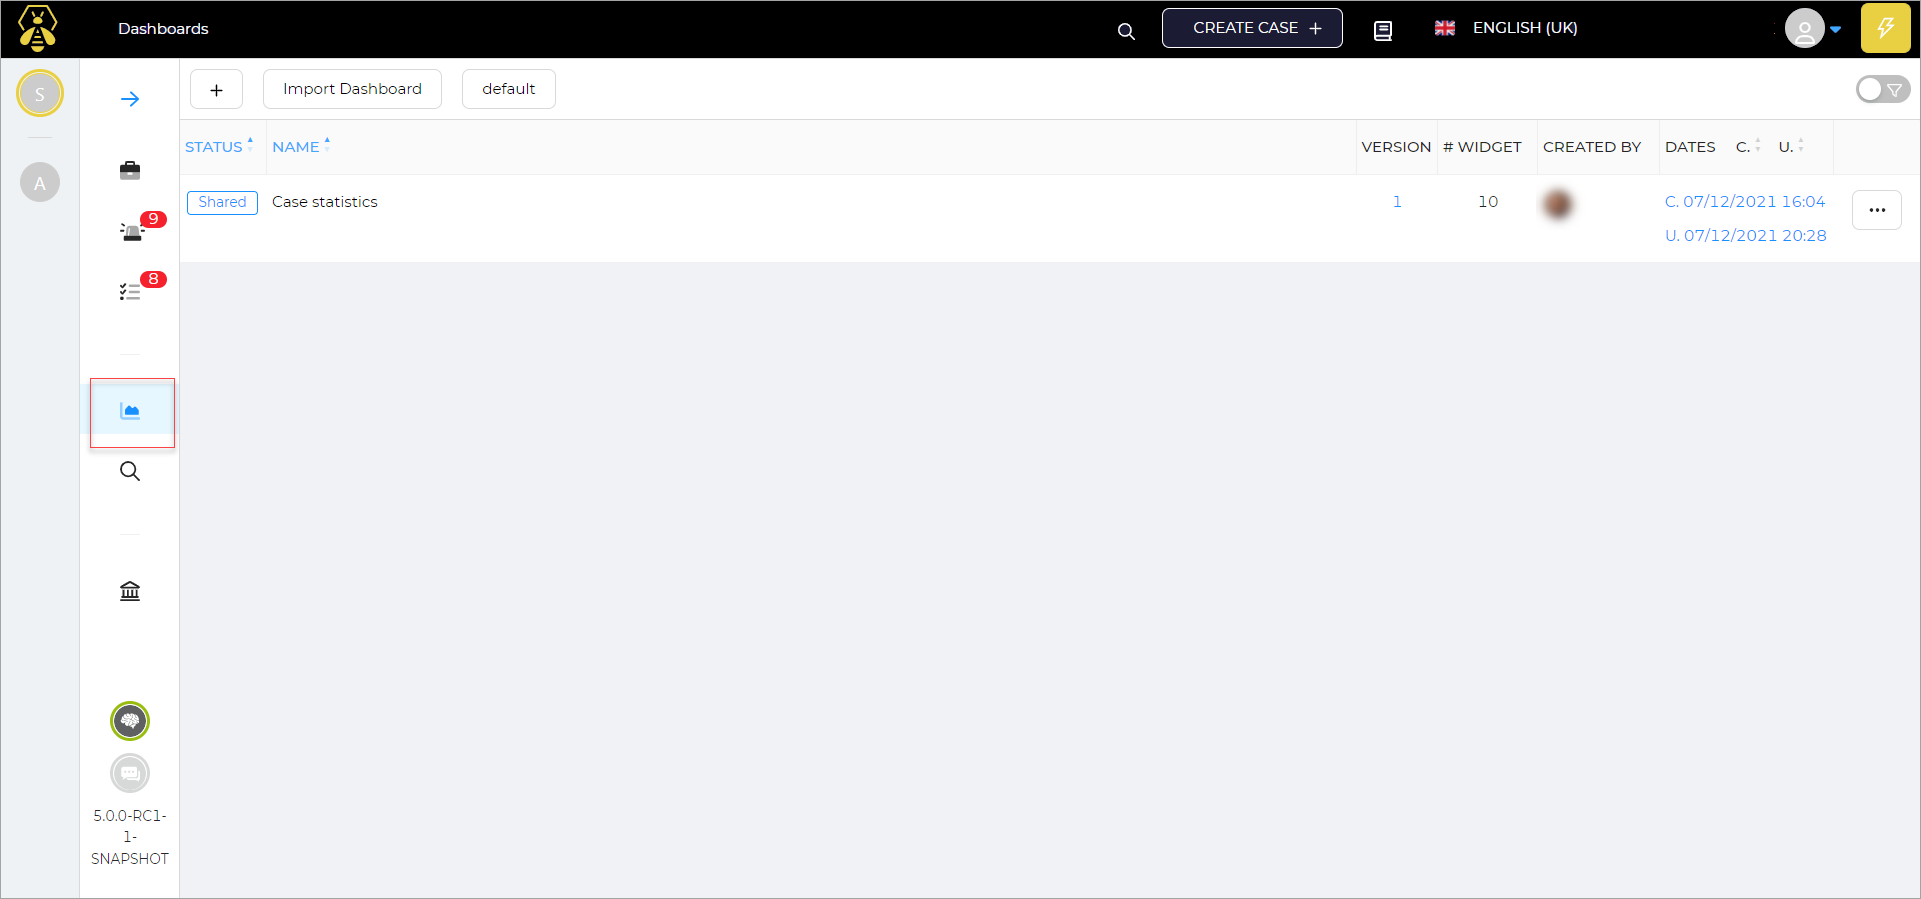
\includegraphics[width=0.8\textwidth]{dashboard1.png}
    \caption{Dashboard}
    \label{fig:dashboard}
\end{figure}

\subsubsection*{Manage Dashboards}

\textbf{Add a dashboard:}

To add a dashboard, follow these steps:

\begin{enumerate}
  \item Click the "+" button to access the "Add Dashboard" menu.
\end{enumerate}

\begin{figure}[H]
    \centering
    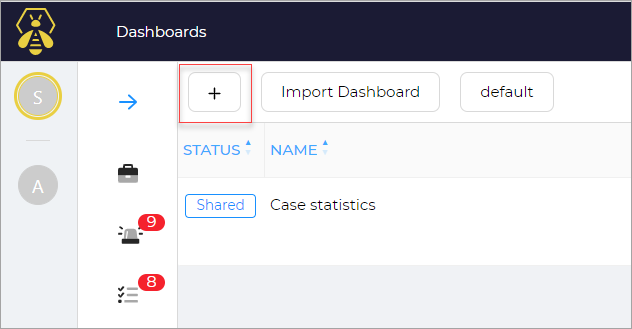
\includegraphics[width=0.8\textwidth]{dashboard2.png}
    \caption{Add Dashboard}
    \label{fig:adddashboard}
\end{figure}

\begin{enumerate}
  \item A new window will open.
  \item Enter the title for the dashboard.
  \item Enter a description for the dashboard.
  \item Select the visibility option (Private or Shared).
  \item Click the "Confirm" button to create the dashboard.
\end{enumerate}

You have successfully added a new dashboard.

\begin{figure}[H]
    \centering
    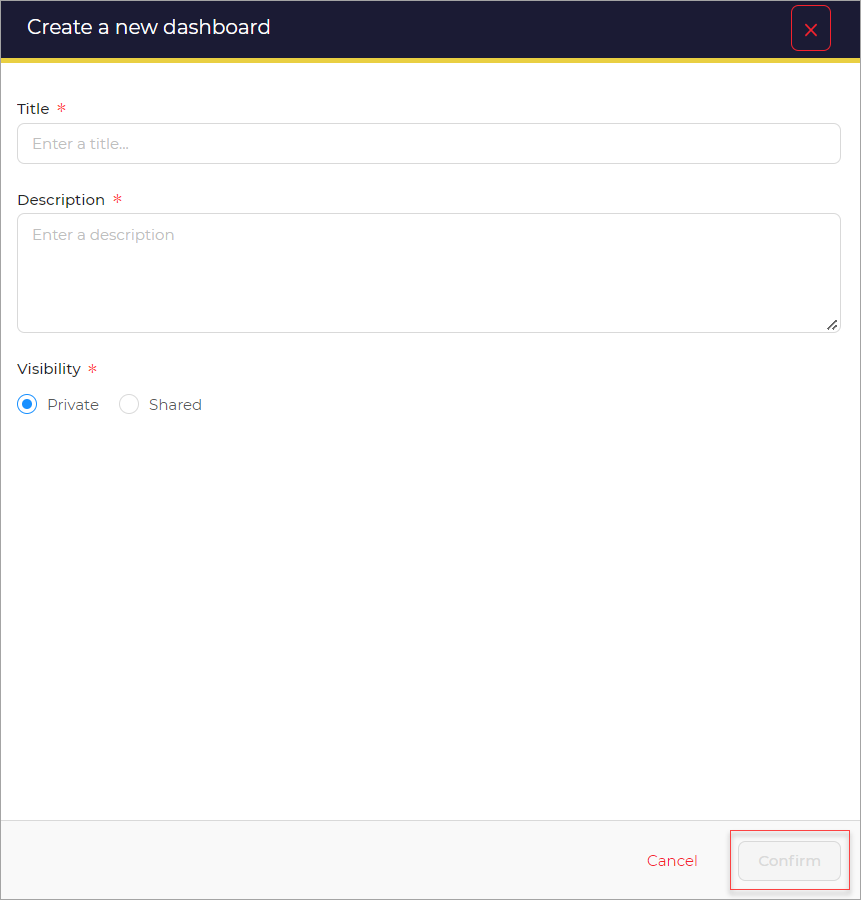
\includegraphics[width=0.8\textwidth]{dashboard3.png}
    \caption{Add Dashboard}
    \label{fig:adddashboard1}
\end{figure}

One can also edit, delete and share dashboards.\\

\subsection{Search}
One can search in the website, by
\begin{itemize}
    \item Cases
    \item Alerts
    \item Observables
    \item Tasks
    \item Jobs
    \item Task logs
\end{itemize}


\section{Powerful Observable Analysis with Cortex}
TheHive offers robust observable analysis capabilities through its integration with Cortex, another powerful tool from TheHive Project. With Cortex, security professionals can conduct in-depth analysis of various types of observables, enhancing incident response efforts through a convenient web interface.

Key features of observable analysis with Cortex include:

\begin{itemize}
  \item \textbf{Extensive Analysis Tools}:
  Cortex provides a wide range of analyzers and responders, allowing you to perform in-depth investigations on various types of observables, such as:
    \begin{itemize}
        \item IP addresses
        \item Email addresses
        \item URLs
        \item Domain names
        \item Files (e.g., attachments)
        \item Hashes (e.g., MD5, SHA-256)
        \item Registry keys (e.g., Windows Registry entries)
        \item And more...
    \end{itemize}
    These tools can reveal crucial information about potential threats associated with these observables.
  
  \item \textbf{Automation}:
  You can automate the analysis process by creating analysis templates that specify which analyzers to run for specific types of observables. This automation streamlines your incident response workflow.
  
  \item \textbf{Scalability}: 
  Cortex is designed to handle a high volume of observables, making it suitable for organizations with large-scale security operations.
  
  \item \textbf{Integration with TheHive}:
  Seamless integration with TheHive means that you can initiate observable analysis directly from your incident cases, improving efficiency and reducing response times.
  
  \item \textbf{Customization}: 
  You can customize Cortex by adding your own analyzers or responders to tailor the analysis capabilities to your organization's specific needs.
\end{itemize}

\subsubsection{Analyzers and Responders}

\begin{figure}[H]
    \centering
    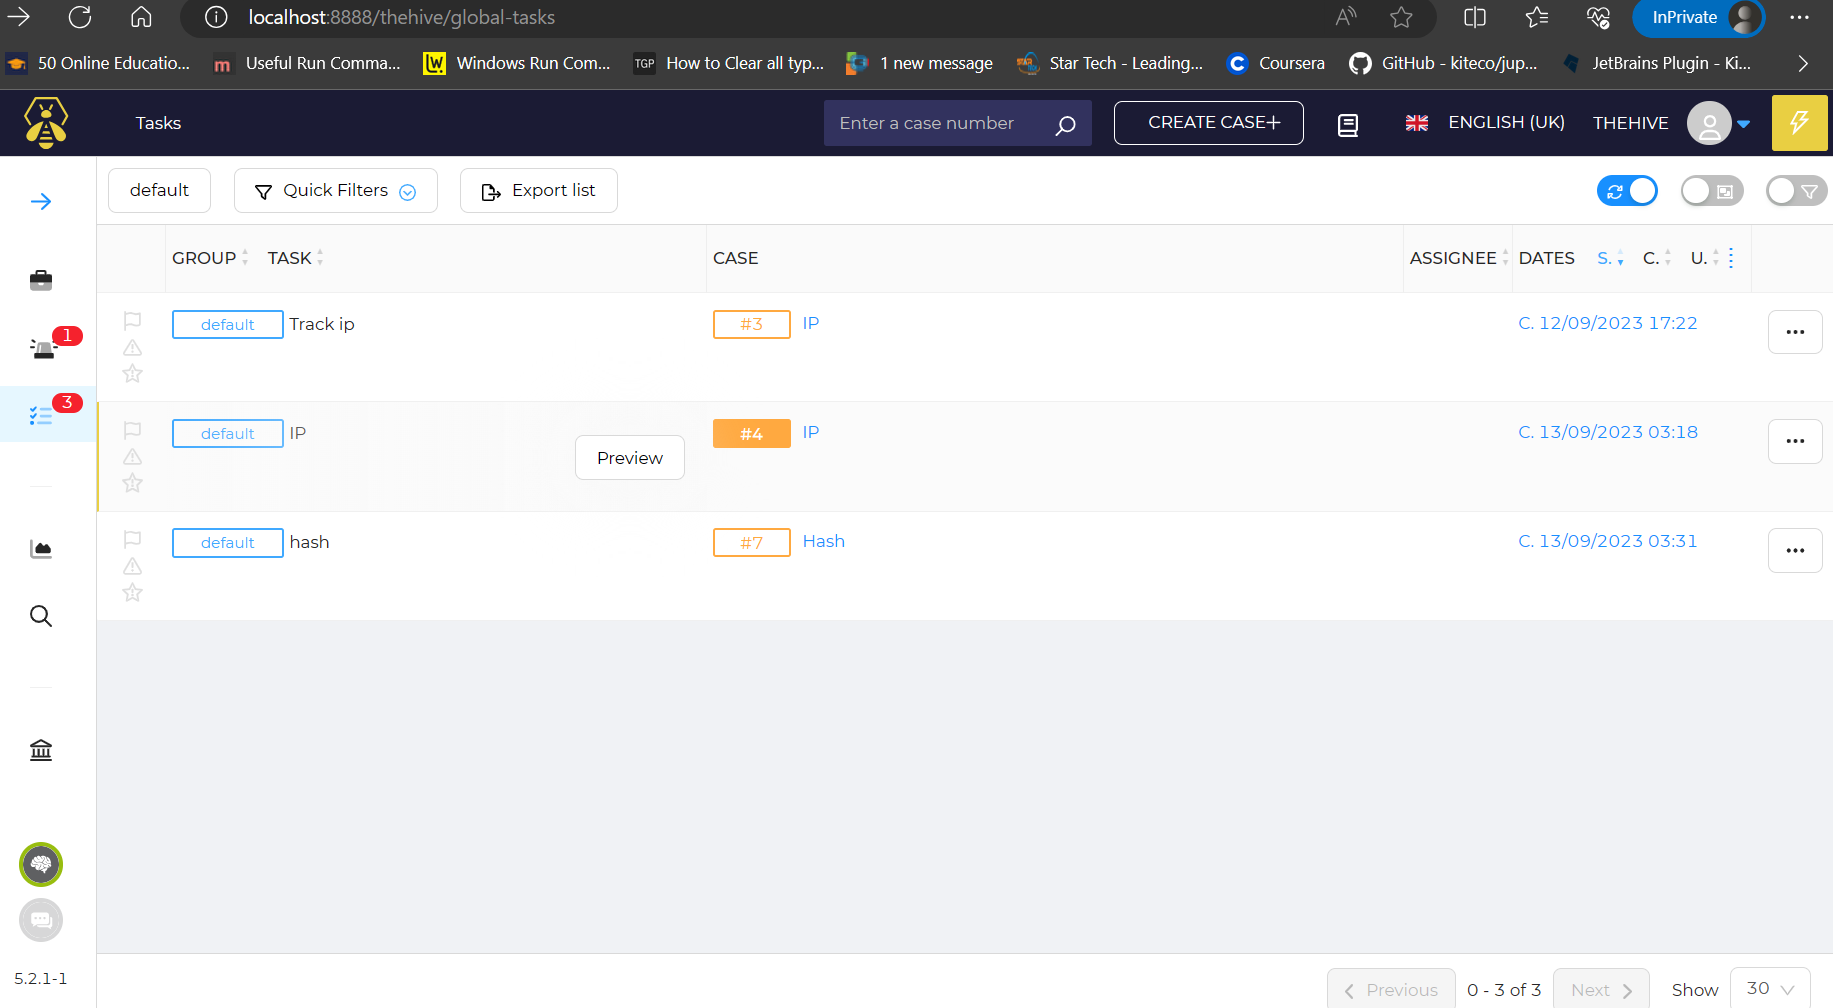
\includegraphics[width=0.8\textwidth]{cases.png}
    \caption{Cases}
    \label{fig:cases}
\end{figure}

\begin{figure}[H]
    \centering
    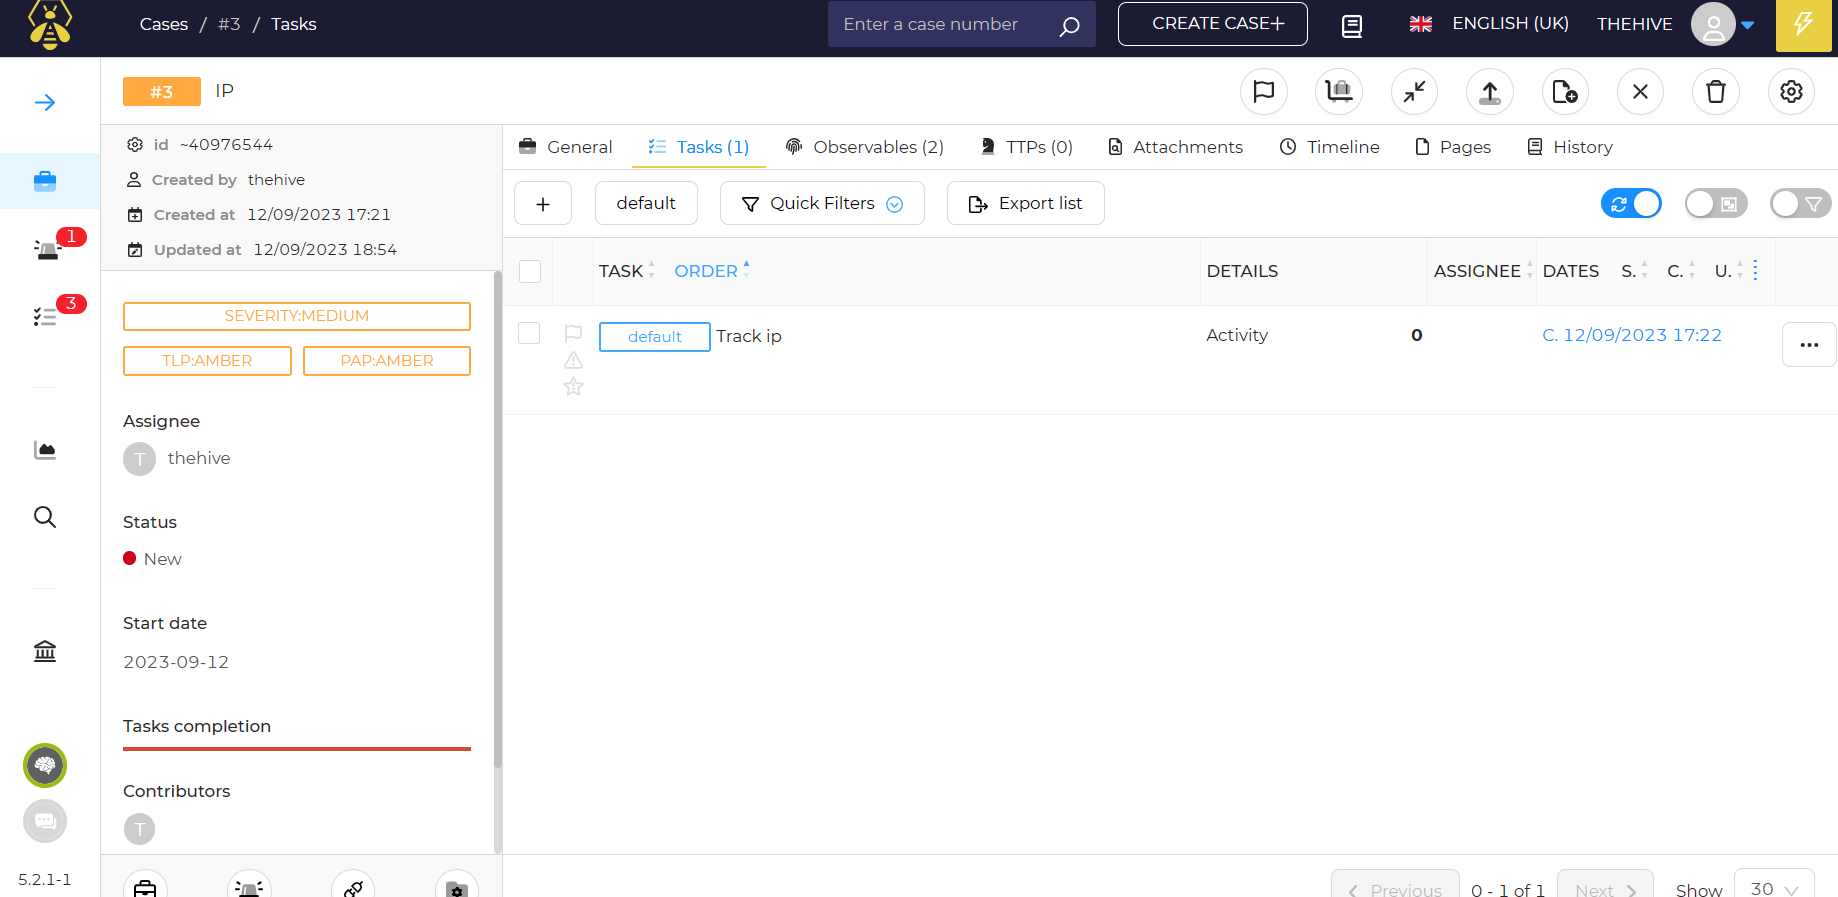
\includegraphics[width=0.8\textwidth]{observables.png}
    \caption{Observables}
    \label{fig:observables}
\end{figure}

Navigating to the case details page, we can see all \textbf{cases} of the organization.
We can see this in Figure \ref{fig:cases}.
Click on the case you want to analyze. And then click on the \textbf{observables} tab of your task.
We can see this in Figure \ref{fig:observables}. Now we can see all the observables of the case and create new observables.
When we want to \textbf{Create Observable} some basic information is required.
\begin{itemize}
    \item \textbf{Type}: Type of the observable.
    \item \textbf{Value}: Value of the observable.
    \item \textbf{Tags}: Tags of the observable, that will help us to search for the observable.
    \item \textbf{Description}
    It is a must to explain what it does.
\end{itemize}

\subsubsection{Analyzers}
\begin{figure}[H]
    \centering
    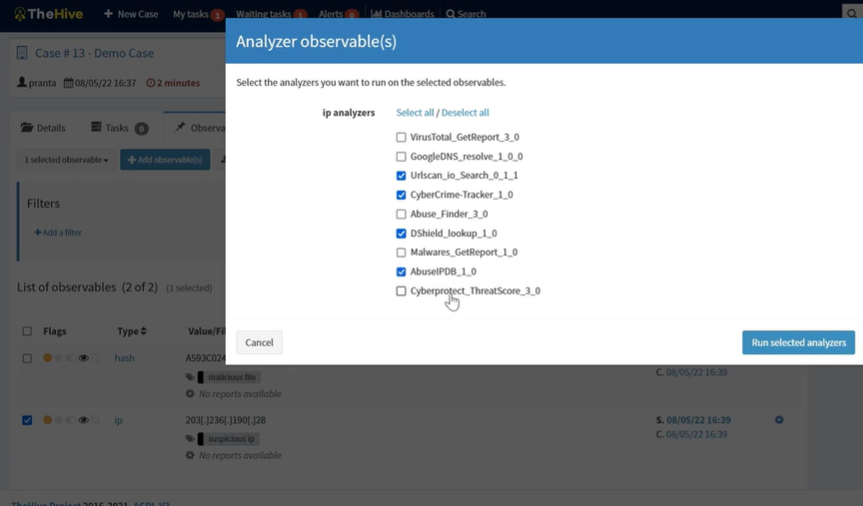
\includegraphics[width=0.8\textwidth]{analyzers.png}
    \caption{Analyzers}
    \label{fig:analyzers}
\end{figure}

\begin{figure}[H]
    \centering
    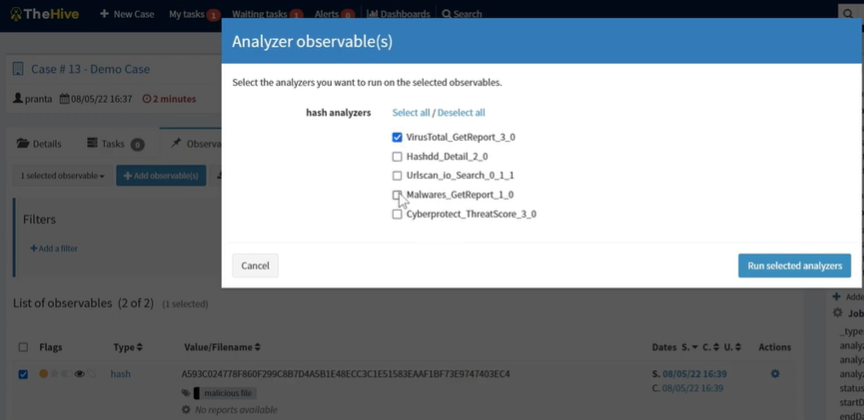
\includegraphics[width=0.8\textwidth]{analyzers2.png}
    \caption{Analyzers}
    \label{fig:analyzers2}
\end{figure}

After creating the observable, we can see the \textbf{analyzers} option. For example, we can see the available analyzers for the IP address observable.
We can see this in Figure \ref{fig:analyzers}.
Here we see the list of analyzers. Cortex provides a wide range of analyzers, as 
\begin{itemize}
    \item \textbf{Abuse Finder}
    \item \textbf{Google DNS Resolver}
    \item \textbf{URL Scan}
    \item \textbf{Cyber Protect Threat Score}
\end{itemize}
Another example is shown in Figure \ref{fig:analyzers2}. Here we can see the available analyzers for hash observable.

\subsubsection{Analysis Report}
After running the analyzer, we can see the analysis report. Here danger levels are shown with results from different analyzers \textbf{Color Coded}.
For example, we can see the analysis report of the hash observable.
We can see 
\begin{figure}[H]
    \centering
    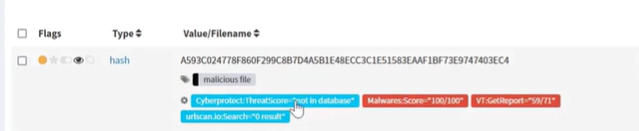
\includegraphics[width=0.8\textwidth]{analyzers-result.png}
    \caption{Analysis Report}
    \label{fig:analysis-report}
\end{figure}
Two blue color means that the hash is not malicious for that analyzer. And two red color means that the hash is malicious for that analyzer.
\section*{Use Cases}
\begin{enumerate}
    \item \textbf{Incident Management:} TheHive allows you to manage your security incidents efficiently by providing a centralized platform for incident management. It enables you to create cases, assign tasks, and track the progress of your investigations.

    \item \textbf{Collaboration:} TheHive allows you to collaborate with other teams and share information about security incidents. You can create alerts, share observables, and communicate with other teams in real-time.

    \item \textbf{Automation:} TheHive allows you to automate your incident response processes by integrating with Cortex. Cortex is a powerful engine that enables you to analyze observables such as IP addresses, email addresses, URLs, domain names, files, or hashes using a web interface. You can also automate these operations and submit large sets of observables from TheHive or through the Cortex REST API from alternative SIRP platforms, custom scripts, or MISP.

    \item \textbf{Reporting:} TheHive provides detailed reports on your incident response activities. You can generate reports on the number of cases created, the number of tasks assigned, and the progress of your investigations.
\end{enumerate}

\section*{Conclusion}
In conclusion, TheHive is a comprehensive platform that provides a range of features to help you manage your security incidents efficiently. It allows you to collaborate with other teams and automate your incident response processes. The platform also provides detailed reports on your incident response activities

\end{document}
